\documentclass[11pt]{article}
\usepackage[T1]{fontenc}
\usepackage[utf8]{inputenc}
\usepackage{lmodern}
\input{glyphtounicode}
\pdfgentounicode=1
\pdftrailerid{}
\usepackage[title]{appendix}
\usepackage{needspace}
\usepackage{amsmath,amssymb,amsthm,geometry,booktabs,tikz,hyperref}
\geometry{margin=1in}
\emergencystretch=1em
\hypersetup{colorlinks=true,linkcolor=blue,citecolor=blue,urlcolor=blue,pdftitle={Locked tromino tilings of rectangles},pdfauthor={P. Graham},pdfsubject={Which rectangles have locked tromino tilings: a proof of Tucker-Foltz's conjecture},pdfkeywords={polyomino tiling, tromino, recombination, ReCom, metagraph, Lean}}
\newtheorem{theorem}{Theorem}
\newtheorem{lemma}[theorem]{Lemma}
\newtheorem{corollary}[theorem]{Corollary}
\newtheorem{proposition}[theorem]{Proposition}
\theoremstyle{definition}
\newtheorem{definition}[theorem]{Definition}
\theoremstyle{remark}
\newtheorem{remark}[theorem]{Remark}
\newcommand{\file}[1]{\texttt{\detokenize{#1}}}
\definecolor{tileA}{RGB}{166,206,227}
\definecolor{tileB}{RGB}{253,205,172}
\definecolor{tileC}{RGB}{204,235,197}
\definecolor{tileD}{RGB}{222,203,228}
\definecolor{tileE}{RGB}{255,242,174}
\definecolor{tileF}{RGB}{230,230,230}
\tikzset{cellgrid/.style={gray!45,very thin},tileedge/.style={black,line width=1.1pt,line cap=round},
  seam/.style={red!80!black,line width=1.6pt,dashed}}
\title{Locked tromino tilings of rectangles}
\author{P. Graham\\ \small\url{https://orcid.org/0009-0007-8493-1505}}
\date{October 28, 2026}
\begin{document}
\maketitle
\begin{abstract}
An $m\times n$ rectangle has a locked tromino tiling if and only if
$3\mid mn$ and $\min(m,n)\ge4$. A tromino consists of three grid cells
connected through shared sides; a tiling is locked if no pair of tiles can
be recombined into a different pair and the rectangle has another tiling.
We prove the existence direction of Tucker-Foltz's conjecture.
Tucker-Foltz showed that rectangles with a side of length at most three
have none, constructed
locked tilings when one side is divisible by three and at least six and
the other is at least one hundred, and conjectured that four suffices.
Following Tucker-Foltz's construction by compatible rectangular blocks,
we supply the remaining cases and glue them along full rows and columns.
Aanjaneya and Pal earlier proved existence on the same rectangles for the
different condition of fault-free L-tromino tilings. Lean formalizes the existence theorem for $3\mid m$, $m\ge6$, $n\ge4$,
including the gluing argument, arithmetic and finite blocks, using only
\texttt{propext}, \texttt{Classical.choice} and \texttt{Quot.sound}.
Two separately written programs, sharing no code, check the blocks and seams.
The classification uses Tucker-Foltz's preprint theorem for narrow
rectangles, whose proof leaves the $m=3$ frontier check to the reader
there; we neither repeat nor formalize that check.
\end{abstract}

\section{Introduction}

Cut a rectangular grid of cells into \emph{trominoes}, sets of three cells
connected through shared sides: straight ones and L-shaped ones, in any
orientation. Pick two of the trominoes, remove them, and try to cover the six
freed cells with two trominoes in a different way. If this is possible the
change is a \emph{recombination move}. A tiling is
\emph{locked} if no recombination move is possible, for any two of its
tiles, although the grid does have other tromino tilings
(Figure~\ref{fig:example}). We determine exactly which rectangles have a
locked tromino tiling.

\begin{theorem}\label{thm:main}
Let $m$ and $n$ be positive integers. The $m\times n$ rectangle has a locked
tromino tiling if and only if $3$ divides $mn$ and $\min(m,n)\ge4$.
\end{theorem}

Tucker-Foltz introduced locked tilings as obstructions to the ReCom Markov
chain of DeFord, Duchin and Solomon~\cite{recom}, which merges two districts
and splits their union into two new ones~\cite[Section~1]{tf}. On a grid
with equal-population cells and three cells per district, plans are tromino
tilings and recombination moves are ReCom steps. Tucker-Foltz proved the
necessary narrow-grid exclusion~\cite[Theorem~3.1]{tf} and existence for
$3\mid m$, $m\ge6$, $n\ge100$~\cite[Theorem~3.2]{tf}, conjecturing that
$n\ge4$ suffices~\cite[Section~3]{tf}.

\begin{theorem}[conjectured by Tucker-Foltz]\label{thm:conj}
Let $m$ and $n$ be integers with $3\mid m$, $m\ge6$ and $n\ge4$. Then the
$m\times n$ rectangle has a locked tromino tiling.
\end{theorem}

The block method is Tucker-Foltz's: the blocks in
\cite[Figure~7 and proof of Theorem~3.2]{tf} cover the family
$m=6u+9v$, $n=22x+19y+8z$, where $u,v,y,z\ge0$, $u+v\ge1$ and $x\ge1$,
and its transposes; in particular they cover $3\mid m$, $m\ge6$, $n\ge100$.
Tucker-Foltz also reports locked tilings of the $6\times4$ rectangle
\cite[Section~3]{tf}; Tucker-Foltz's $6\times6$ example extends by flipped copies
to every $6r\times6s$, $r,s\ge1$ \cite[Section~1, Figures~2--3]{tf}. Our blocks cover all the
rectangles in Theorem~\ref{thm:conj}, including the remaining cases. We use
compatible blocks as in Tucker-Foltz's construction. The difficult step
is finding blocks at narrow widths that remain rigid against one another
in both orders and against copies of themselves. Section~\ref{sec:overview}
explains how finitely many such blocks suffice. The existence proof,
including their compatibility, is formalized in Lean~4~\cite{lean}.

Up to transposition, the smallest permitted rectangles by area are $6\times4$,
$6\times5$, $6\times6$ and $9\times4$; only the $6\times4$ and $6\times6$
cases among these four were settled before~\cite[Sections~1 and~3]{tf}. This classification concerns
the grid model with three-cell districts. Related irreducibility results
include Cannon's theorem for three simply connected districts in a
triangular region of the triangular lattice, allowing district sizes to
vary by at most one vertex~\cite{cannon}. Akitaya, Dituro, Gonczi,
Korman, Souvaine, Stock and T\'oth simplify the proof, weaken Cannon's
hypotheses, and prove a square-grid analogue~\cite{akitaya}; both allow
size tolerance, as discussed in \cite[Section~1.2]{emre}. Emre, Jerison
and Veomett prove connectivity for a $3\times n$ grid with three
districts of size $n$~\cite[Theorem~3]{emre}.

Aanjaneya and Pal~\cite[Theorem~2]{faultfree} proved that every rectangle
with $m,n\ge4$ and $3\mid mn$ admits a fault-free L-tromino tiling,
also by extending finitely
many small rectangles. A fault line is a full horizontal or vertical cut
that crosses no tile; fault-free means no such cut exists. Locked tilings
instead forbid two-tile recombinations and allow straight and L-trominoes.
These are different conditions: tilings assembled from multiple blocks
have fault lines along their joins, while lockedness concerns two-tile recombinations.

The proofs, the Lean formalization, the certificate checkers and the text
were produced by AI models (from OpenAI and Anthropic), working under the
author's direction. This work has not yet been reviewed by experts.

\begin{figure}[ht]
\centering
%% BEGIN FIGURE example
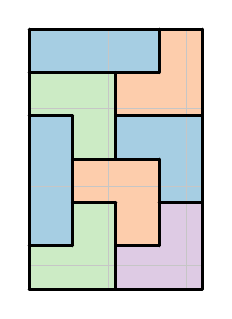
\begin{tikzpicture}[x=0.55cm,y=0.55cm]
\fill[tileA] (0,0) rectangle ++(1,-1);
\fill[tileA] (1,0) rectangle ++(1,-1);
\fill[tileA] (2,0) rectangle ++(1,-1);
\fill[tileB] (3,0) rectangle ++(1,-1);
\fill[tileB] (2,-1) rectangle ++(1,-1);
\fill[tileB] (3,-1) rectangle ++(1,-1);
\fill[tileC] (0,-1) rectangle ++(1,-1);
\fill[tileC] (1,-1) rectangle ++(1,-1);
\fill[tileC] (1,-2) rectangle ++(1,-1);
\fill[tileA] (0,-2) rectangle ++(1,-1);
\fill[tileA] (0,-3) rectangle ++(1,-1);
\fill[tileA] (0,-4) rectangle ++(1,-1);
\fill[tileA] (2,-2) rectangle ++(1,-1);
\fill[tileA] (3,-2) rectangle ++(1,-1);
\fill[tileA] (3,-3) rectangle ++(1,-1);
\fill[tileB] (1,-3) rectangle ++(1,-1);
\fill[tileB] (2,-3) rectangle ++(1,-1);
\fill[tileB] (2,-4) rectangle ++(1,-1);
\fill[tileC] (1,-4) rectangle ++(1,-1);
\fill[tileC] (0,-5) rectangle ++(1,-1);
\fill[tileC] (1,-5) rectangle ++(1,-1);
\fill[tileD] (3,-4) rectangle ++(1,-1);
\fill[tileD] (2,-5) rectangle ++(1,-1);
\fill[tileD] (3,-5) rectangle ++(1,-1);
\draw[cellgrid] (0,0) grid (4,-6);
\draw[tileedge] (0,-1)--++(1,0) (1,-1)--++(1,0) (3,0)--++(0,-1) (2,-1)--++(1,0) (4,0)--++(0,-1) (0,-2)--++(1,0) (2,-1)--++(0,-1) (2,-2)--++(1,0);
\draw[tileedge] (4,-1)--++(0,-1) (3,-2)--++(1,0) (1,-2)--++(0,-1) (2,-2)--++(0,-1) (1,-3)--++(1,0) (2,-3)--++(1,0) (4,-2)--++(0,-1) (1,-3)--++(0,-1);
\draw[tileedge] (1,-4)--++(1,0) (3,-3)--++(0,-1) (4,-3)--++(0,-1) (3,-4)--++(1,0) (1,-4)--++(0,-1) (0,-5)--++(1,0) (2,-4)--++(0,-1) (3,-4)--++(0,-1);
\draw[tileedge] (2,-5)--++(1,0) (4,-4)--++(0,-1) (0,-6)--++(1,0) (2,-5)--++(0,-1) (1,-6)--++(1,0) (2,-6)--++(1,0) (4,-5)--++(0,-1) (3,-6)--++(1,0);
\draw[tileedge] (0,0)--++(0,-1) (0,-1)--++(0,-1) (0,-2)--++(0,-1) (0,-3)--++(0,-1) (0,-4)--++(0,-1) (0,-5)--++(0,-1) (0,0)--++(1,0) (1,0)--++(1,0);
\draw[tileedge] (2,0)--++(1,0) (3,0)--++(1,0);
\end{tikzpicture}
%% END FIGURE example
\caption{A locked tromino tiling of the $6\times4$ rectangle. Thick lines
are tile boundaries; colors only separate neighboring tiles. It is the
height-6 block of width 4 used in the proof.}
\label{fig:example}
\end{figure}

\section{Tilings and rigidity}\label{sec:defs}

A \emph{cell} is a pair of integers $(i,j)$, read as row $i$ and column $j$.
Two cells are \emph{adjacent} if they agree in one coordinate and differ by
one in the other. The $m\times n$ \emph{rectangle} is the set of cells
$(i,j)$ with $0\le i<m$ and $0\le j<n$; it has $m$ rows and $n$ columns. A
\emph{tromino} is a set of three cells that is connected: any two of its
cells are joined by a sequence of adjacent cells inside it. Up to
translation there are six trominoes, two straight and four L-shaped. A
\emph{tiling} of a set of cells is a partition of it into trominoes, called
its \emph{tiles}.

\begin{definition}\label{def:locked}
Let $T$ be a tiling and $A,B$ two of its tiles. A \emph{recombination move}
on $\{A,B\}$ replaces them by two disjoint trominoes $C,D$ with
$C\cup D=A\cup B$ and $\{C,D\}\ne\{A,B\}$. The pair $\{A,B\}$ is
\emph{rigid} if it admits no recombination move. The tiling $T$ of a
rectangle is \emph{locked} if every pair of its tiles is rigid and the
rectangle has a tiling other than $T$.
\end{definition}

Tucker-Foltz~\cite[Section~1]{tf} works with the \emph{metagraph}
$M(G,3)$ of a graph $G$: its vertices are the partitions of $G$ into
connected subgraphs of three vertices each, and two partitions are adjacent
when they differ only on two parts. A locked tiling is an isolated vertex of
$M(G,3)$ that is not its only vertex. For the grid graph $G$ of a rectangle,
the vertices are the tromino tilings, and two tilings that differ only on two
parts cover the same six cells with those parts, so its edges are exactly the
recombination moves. The two definitions of a locked tiling therefore agree.

Translating a tiling, or reflecting it in a horizontal, vertical or diagonal
line, preserves adjacency, so it maps trominoes to trominoes, recombination
moves to recombination moves and locked tilings to locked tilings. In
particular the transpose $(i,j)\mapsto(j,i)$ turns locked tilings of the
$m\times n$ rectangle into locked tilings of the $n\times m$ rectangle.

\begin{lemma}\label{lem:apart}
Let $A$ and $B$ be disjoint trominoes such that no cell of $A$ is adjacent
to a cell of $B$. Then $\{A,B\}$ is rigid.
\end{lemma}

\begin{proof}
Let $C$ and $D$ be disjoint trominoes with $C\cup D=A\cup B$. A path of
adjacent cells inside $A\cup B$ that starts in $A$ never reaches $B$, because
its first step into $B$ would join a cell of $A$ to an adjacent cell of $B$.
Since $C$ is connected, it therefore lies inside $A$ or inside $B$, and
since all three sets have three cells, $C$ equals $A$ or $B$. The same holds
for $D$, and $C\ne D$ because they are disjoint and nonempty. Hence
$\{C,D\}=\{A,B\}$.
\end{proof}

\begin{lemma}\label{lem:two}
If $m$ and $n$ are positive integers with $3\mid m$ and $n\ge3$, the $m\times n$ rectangle has at least two tromino
tilings. Hence a tiling of it is locked as soon as every pair of its tiles is
rigid.
\end{lemma}

\begin{proof}
Cover every column by vertical straight trominoes; or cover the first three
columns by horizontal straight trominoes, one in each row, and the remaining
columns by vertical ones (Figure~\ref{fig:two}). The second tiling contains
the tile $\{(0,0),(0,1),(0,2)\}$ and the first does not. Any tiling differs
from at least one of the two.
\end{proof}


The necessary condition uses Tucker-Foltz's narrow-grid theorem, stated in
that paper's notation: $G(m,n)$ is the $m\times n$ grid graph.

\begin{theorem}[{Tucker-Foltz~\cite[Theorem~3.1]{tf}}]\label{thm:narrow}
For any positive integers $m$ and $n$ such that $m\le3$, $M(G(m,n),3)$ is
connected.
\end{theorem}

For $m=3$, Tucker-Foltz's proof reduces to an exhaustive list of frontier
configurations (their Figure~6), whose verification is left to the reader
there; we neither repeat it nor formalize it.


\section{Proof overview}\label{sec:overview}

By Lemma~\ref{lem:two}, it suffices to construct a tiling with every pair
rigid. We cut along full rows and columns into rectangular blocks. The
gluing lemma shows that recombination can occur only within a block or
across a shared side, called a seam. It therefore suffices to choose rigid
blocks whose seams are rigid for both orders, including repeated blocks (the directional conventions are defined in
Section~\ref{sec:glue}).

Heights 6 and 9 generate every multiple of three from six onward. At each
width from 4 to 55, one column of blocks suffices, except that width 5 uses
heights 9 and 12 and separate tilings at heights 6 and 15, which are not
sums of nines and twelves. For widths at
least 56, sums of eights and nines allow a grid built from four block types with heights
6 and 9 and widths 8 and 9. We prove the gluing assertion, state the finite
construction, and then assemble the tilings using these arithmetic facts.

\section{Gluing rectangular blocks}\label{sec:glue}

Let $m=h_1+\dots+h_r$ and $n=w_1+\dots+w_s$ with positive integers $h_k$ and
$w_l$. Put $H_k=h_1+\dots+h_k$ and $W_l=w_1+\dots+w_l$, with $H_0=W_0=0$. The
\emph{block} $(k,l)$ is the set of cells $(i,j)$ with $H_{k-1}\le i<H_k$ and
$W_{l-1}\le j<W_l$, an $h_k\times w_l$ rectangle. The blocks partition the
$m\times n$ rectangle. Two blocks are \emph{side neighbors} if they lie in
the same row of blocks and in consecutive columns of blocks, or in the same
column of blocks and in consecutive rows of blocks.

\begin{lemma}[gluing]\label{lem:glue}
For each block $(k,l)$ let $T_{kl}$ be a tiling of it, and let $T$ be the
union of these tilings, a tiling of the $m\times n$ rectangle. Suppose that
\begin{enumerate}
\item[(a)] every pair of tiles of each $T_{kl}$ is rigid, and
\item[(b)] for every two side neighbors $(k,l)$ and $(k',l')$, every pair
consisting of a tile of $T_{kl}$ and a tile of $T_{k'l'}$ is rigid.
\end{enumerate}
Then every pair of tiles of $T$ is rigid.
\end{lemma}

\begin{proof}
Let $A$ and $B$ be tiles of $T$, in blocks $(k,l)$ and $(k',l')$. If the
blocks are equal or side neighbors, $\{A,B\}$ is rigid by (a) or (b).
Otherwise we show that no cell of $A$ is adjacent to a cell of $B$, so that
Lemma~\ref{lem:apart} applies. Let $(i,j)\in A$ and $(i',j')\in B$ be
adjacent. Then $|i-i'|\le1$, and since every height $h_k$ is positive, the
rows $i$ and $i'$ lie in the same row of blocks or in consecutive ones; the
same holds for the columns $j$ and $j'$. Adjacent cells also agree in one
coordinate, so the two blocks share a row of blocks or a column of blocks.
Hence they are equal or side neighbors, contrary to assumption.
\end{proof}

Condition (b) concerns only two blocks at a time, and rigidity is unchanged
by translation, so it can be checked on a fixed pair of rectangles. For a
tiling $X$ of an $h\times w$ rectangle and a tiling $Y$ of an $h'\times w$
rectangle, say that $X$ \emph{stacks on} $Y$ if, after $Y$ is moved down by
$h$ rows, every tile of $X$ forms a rigid pair with every tile of the moved
$Y$; the line between them is the seam. Similarly, for equal heights, $X$
\emph{fits left of} $Y$ if this holds after $Y$ is moved right by the width
of $X$. We also call a rectangular tiling a block when its tile partition is
understood. A tiling or block is \emph{rigid} if all pairs of its tiles are.
Figure~\ref{fig:stack} shows the four stacks of the two width-4 blocks, and
Figure~\ref{fig:palette} the four blocks for large widths, with both kinds of
seam.

\begin{corollary}\label{cor:assemble}
\begin{enumerate}
\item[(i)] Let $S$ be a set of rigid blocks of a common width $w$ such that
every $X\in S$ stacks on every $Y\in S$, including $Y=X$. Then any column of
blocks from $S$, placed one under another, is a tiling of an $h\times w$
rectangle all of whose pairs of tiles are rigid, where $h$ is the sum of the
heights.
\item[(ii)] Let $P_{h,w}$, for $h$ in a set $\mathcal H$ and $w$ in a set
$\mathcal W$, be rigid blocks of size $h\times w$ such that $P_{h,w}$ stacks
on $P_{h',w}$ and fits left of $P_{h,w'}$ for all $h,h'\in\mathcal H$ and
$w,w'\in\mathcal W$. If $m=h_1+\dots+h_r$ with every $h_k\in\mathcal H$ and
$n=w_1+\dots+w_s$ with every $w_l\in\mathcal W$, the tiling that places a
translate of $P_{h_k,w_l}$ in block $(k,l)$ has only rigid pairs.
\end{enumerate}
\end{corollary}

\begin{proof}
Both follow from Lemma~\ref{lem:glue}. In (ii), condition (a) is the rigidity of the
blocks, and for side neighbors $(k,l)$ above $(k+1,l)$ or left of $(k,l+1)$,
condition (b) is the statement that $P_{h_k,w_l}$ stacks on
$P_{h_{k+1},w_l}$ or fits left of $P_{h_k,w_{l+1}}$, translated into place.
Part (i) is the case of a single column of blocks.
\end{proof}

\section{The block construction}\label{sec:blocks}

The blocks were found by a SAT encoding of tile placements and forbidden
recombinations. Their coordinates are in the \file{data/} folder released
with this paper (Appendix~\ref{app:data}), archived at
\url{https://doi.org/10.5281/zenodo.23638798}~\cite{GrahamArchive}.
For each block, the finite verification establishes
that the cells are partitioned into connected triples. It then enumerates
every partition of the six cells of a pair of tiles into two connected
triples, checking that only the original pair occurs. This is done inside
each block and across every listed seam; pairs with no adjacent cells are
rigid by Lemma~\ref{lem:apart}.

\Needspace{7\baselineskip}
\begin{proposition}\label{prop:blocks}
The following tilings exist and are given explicitly in the \file{data/}
folder (Appendix~\ref{app:data}).
\begin{enumerate}
\item[(i)] For each width $w$ with $4\le w\le55$ and $w\ne5$, rigid blocks
$B_{6,w}$ and $B_{9,w}$ of sizes $6\times w$ and $9\times w$, each of which
stacks on each, including itself.
\item[(ii)] Rigid blocks $B_{9,5}$ and $B_{12,5}$ of sizes $9\times5$ and
$12\times5$, each of which stacks on each, including itself; and rigid
tilings of the $6\times5$ and $15\times5$ rectangles.
\item[(iii)] Rigid blocks $P_{h,w}$ of size $h\times w$ for $h\in\{6,9\}$
and $w\in\{8,9\}$, such that $P_{h,w}$ stacks on $P_{h',w}$ and fits left of
$P_{h,w'}$ for all $h,h'\in\{6,9\}$ and $w,w'\in\{8,9\}$.
\end{enumerate}
\end{proposition}

The width-5 construction uses heights 9 and 12; no nonexistence claim for
a compatible height-6 block is needed or established here.

Figures~\ref{fig:stack}, \ref{fig:palette} and~\ref{fig:five} show the
width-4 blocks, the four blocks for large widths and the width-5 tilings.
\begin{proof}
Each statement is a finite check of explicit tilings: that each block is a
tiling of its rectangle by trominoes, and that each of the listed pairs of
tiles, inside a block or across a seam, admits only its own partition into
two trominoes. Lean's kernel checks all of them, and so do two separately
written programs (Section~\ref{sec:formal}).
\end{proof}

\begin{figure}[ht]
\centering
%% BEGIN FIGURE stack
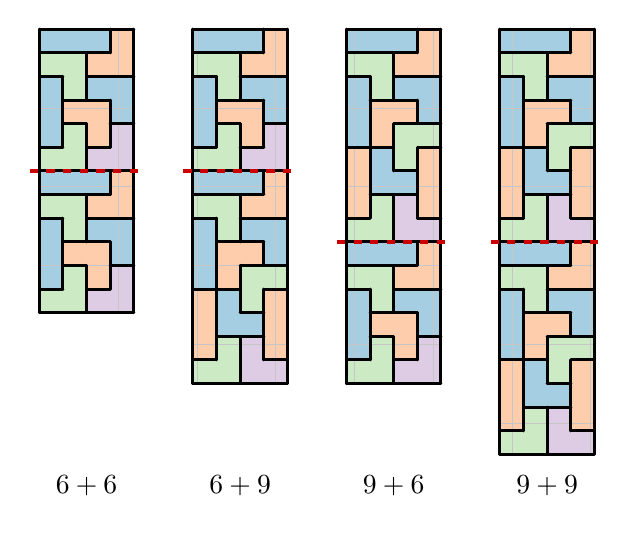
\begin{tikzpicture}[x=0.3cm,y=0.3cm]
\fill[tileA] (0,0) rectangle ++(1,-1);
\fill[tileA] (1,0) rectangle ++(1,-1);
\fill[tileA] (2,0) rectangle ++(1,-1);
\fill[tileB] (3,0) rectangle ++(1,-1);
\fill[tileB] (2,-1) rectangle ++(1,-1);
\fill[tileB] (3,-1) rectangle ++(1,-1);
\fill[tileC] (0,-1) rectangle ++(1,-1);
\fill[tileC] (1,-1) rectangle ++(1,-1);
\fill[tileC] (1,-2) rectangle ++(1,-1);
\fill[tileA] (0,-2) rectangle ++(1,-1);
\fill[tileA] (0,-3) rectangle ++(1,-1);
\fill[tileA] (0,-4) rectangle ++(1,-1);
\fill[tileA] (2,-2) rectangle ++(1,-1);
\fill[tileA] (3,-2) rectangle ++(1,-1);
\fill[tileA] (3,-3) rectangle ++(1,-1);
\fill[tileB] (1,-3) rectangle ++(1,-1);
\fill[tileB] (2,-3) rectangle ++(1,-1);
\fill[tileB] (2,-4) rectangle ++(1,-1);
\fill[tileC] (1,-4) rectangle ++(1,-1);
\fill[tileC] (0,-5) rectangle ++(1,-1);
\fill[tileC] (1,-5) rectangle ++(1,-1);
\fill[tileD] (3,-4) rectangle ++(1,-1);
\fill[tileD] (2,-5) rectangle ++(1,-1);
\fill[tileD] (3,-5) rectangle ++(1,-1);
\fill[tileA] (0,-6) rectangle ++(1,-1);
\fill[tileA] (1,-6) rectangle ++(1,-1);
\fill[tileA] (2,-6) rectangle ++(1,-1);
\fill[tileB] (3,-6) rectangle ++(1,-1);
\fill[tileB] (2,-7) rectangle ++(1,-1);
\fill[tileB] (3,-7) rectangle ++(1,-1);
\fill[tileC] (0,-7) rectangle ++(1,-1);
\fill[tileC] (1,-7) rectangle ++(1,-1);
\fill[tileC] (1,-8) rectangle ++(1,-1);
\fill[tileA] (0,-8) rectangle ++(1,-1);
\fill[tileA] (0,-9) rectangle ++(1,-1);
\fill[tileA] (0,-10) rectangle ++(1,-1);
\fill[tileA] (2,-8) rectangle ++(1,-1);
\fill[tileA] (3,-8) rectangle ++(1,-1);
\fill[tileA] (3,-9) rectangle ++(1,-1);
\fill[tileB] (1,-9) rectangle ++(1,-1);
\fill[tileB] (2,-9) rectangle ++(1,-1);
\fill[tileB] (2,-10) rectangle ++(1,-1);
\fill[tileC] (1,-10) rectangle ++(1,-1);
\fill[tileC] (0,-11) rectangle ++(1,-1);
\fill[tileC] (1,-11) rectangle ++(1,-1);
\fill[tileD] (3,-10) rectangle ++(1,-1);
\fill[tileD] (2,-11) rectangle ++(1,-1);
\fill[tileD] (3,-11) rectangle ++(1,-1);
\draw[cellgrid] (0,0) grid (4,-12);
\draw[tileedge] (0,-1)--++(1,0) (1,-1)--++(1,0) (3,0)--++(0,-1) (2,-1)--++(1,0) (4,0)--++(0,-1) (0,-2)--++(1,0) (2,-1)--++(0,-1) (2,-2)--++(1,0);
\draw[tileedge] (4,-1)--++(0,-1) (3,-2)--++(1,0) (1,-2)--++(0,-1) (2,-2)--++(0,-1) (1,-3)--++(1,0) (2,-3)--++(1,0) (4,-2)--++(0,-1) (1,-3)--++(0,-1);
\draw[tileedge] (1,-4)--++(1,0) (3,-3)--++(0,-1) (4,-3)--++(0,-1) (3,-4)--++(1,0) (1,-4)--++(0,-1) (0,-5)--++(1,0) (2,-4)--++(0,-1) (3,-4)--++(0,-1);
\draw[tileedge] (2,-5)--++(1,0) (4,-4)--++(0,-1) (0,-6)--++(1,0) (2,-5)--++(0,-1) (1,-6)--++(1,0) (2,-6)--++(1,0) (4,-5)--++(0,-1) (3,-6)--++(1,0);
\draw[tileedge] (0,-7)--++(1,0) (1,-7)--++(1,0) (3,-6)--++(0,-1) (2,-7)--++(1,0) (4,-6)--++(0,-1) (0,-8)--++(1,0) (2,-7)--++(0,-1) (2,-8)--++(1,0);
\draw[tileedge] (4,-7)--++(0,-1) (3,-8)--++(1,0) (1,-8)--++(0,-1) (2,-8)--++(0,-1) (1,-9)--++(1,0) (2,-9)--++(1,0) (4,-8)--++(0,-1) (1,-9)--++(0,-1);
\draw[tileedge] (1,-10)--++(1,0) (3,-9)--++(0,-1) (4,-9)--++(0,-1) (3,-10)--++(1,0) (1,-10)--++(0,-1) (0,-11)--++(1,0) (2,-10)--++(0,-1) (3,-10)--++(0,-1);
\draw[tileedge] (2,-11)--++(1,0) (4,-10)--++(0,-1) (0,-12)--++(1,0) (2,-11)--++(0,-1) (1,-12)--++(1,0) (2,-12)--++(1,0) (4,-11)--++(0,-1) (3,-12)--++(1,0);
\draw[tileedge] (0,0)--++(0,-1) (0,-1)--++(0,-1) (0,-2)--++(0,-1) (0,-3)--++(0,-1) (0,-4)--++(0,-1) (0,-5)--++(0,-1) (0,-6)--++(0,-1) (0,-7)--++(0,-1);
\draw[tileedge] (0,-8)--++(0,-1) (0,-9)--++(0,-1) (0,-10)--++(0,-1) (0,-11)--++(0,-1) (0,0)--++(1,0) (1,0)--++(1,0) (2,0)--++(1,0) (3,0)--++(1,0);
\draw[seam] (-0.4,-6)--(4.4,-6);
\node[below] at (2,-18.5) {$6+6$};
\fill[tileA] (6.5,0) rectangle ++(1,-1);
\fill[tileA] (7.5,0) rectangle ++(1,-1);
\fill[tileA] (8.5,0) rectangle ++(1,-1);
\fill[tileB] (9.5,0) rectangle ++(1,-1);
\fill[tileB] (8.5,-1) rectangle ++(1,-1);
\fill[tileB] (9.5,-1) rectangle ++(1,-1);
\fill[tileC] (6.5,-1) rectangle ++(1,-1);
\fill[tileC] (7.5,-1) rectangle ++(1,-1);
\fill[tileC] (7.5,-2) rectangle ++(1,-1);
\fill[tileA] (6.5,-2) rectangle ++(1,-1);
\fill[tileA] (6.5,-3) rectangle ++(1,-1);
\fill[tileA] (6.5,-4) rectangle ++(1,-1);
\fill[tileA] (8.5,-2) rectangle ++(1,-1);
\fill[tileA] (9.5,-2) rectangle ++(1,-1);
\fill[tileA] (9.5,-3) rectangle ++(1,-1);
\fill[tileB] (7.5,-3) rectangle ++(1,-1);
\fill[tileB] (8.5,-3) rectangle ++(1,-1);
\fill[tileB] (8.5,-4) rectangle ++(1,-1);
\fill[tileC] (7.5,-4) rectangle ++(1,-1);
\fill[tileC] (6.5,-5) rectangle ++(1,-1);
\fill[tileC] (7.5,-5) rectangle ++(1,-1);
\fill[tileD] (9.5,-4) rectangle ++(1,-1);
\fill[tileD] (8.5,-5) rectangle ++(1,-1);
\fill[tileD] (9.5,-5) rectangle ++(1,-1);
\fill[tileA] (6.5,-6) rectangle ++(1,-1);
\fill[tileA] (7.5,-6) rectangle ++(1,-1);
\fill[tileA] (8.5,-6) rectangle ++(1,-1);
\fill[tileB] (9.5,-6) rectangle ++(1,-1);
\fill[tileB] (8.5,-7) rectangle ++(1,-1);
\fill[tileB] (9.5,-7) rectangle ++(1,-1);
\fill[tileC] (6.5,-7) rectangle ++(1,-1);
\fill[tileC] (7.5,-7) rectangle ++(1,-1);
\fill[tileC] (7.5,-8) rectangle ++(1,-1);
\fill[tileA] (6.5,-8) rectangle ++(1,-1);
\fill[tileA] (6.5,-9) rectangle ++(1,-1);
\fill[tileA] (6.5,-10) rectangle ++(1,-1);
\fill[tileA] (8.5,-8) rectangle ++(1,-1);
\fill[tileA] (9.5,-8) rectangle ++(1,-1);
\fill[tileA] (9.5,-9) rectangle ++(1,-1);
\fill[tileB] (7.5,-9) rectangle ++(1,-1);
\fill[tileB] (8.5,-9) rectangle ++(1,-1);
\fill[tileB] (7.5,-10) rectangle ++(1,-1);
\fill[tileC] (8.5,-10) rectangle ++(1,-1);
\fill[tileC] (9.5,-10) rectangle ++(1,-1);
\fill[tileC] (8.5,-11) rectangle ++(1,-1);
\fill[tileB] (6.5,-11) rectangle ++(1,-1);
\fill[tileB] (6.5,-12) rectangle ++(1,-1);
\fill[tileB] (6.5,-13) rectangle ++(1,-1);
\fill[tileA] (7.5,-11) rectangle ++(1,-1);
\fill[tileA] (7.5,-12) rectangle ++(1,-1);
\fill[tileA] (8.5,-12) rectangle ++(1,-1);
\fill[tileB] (9.5,-11) rectangle ++(1,-1);
\fill[tileB] (9.5,-12) rectangle ++(1,-1);
\fill[tileB] (9.5,-13) rectangle ++(1,-1);
\fill[tileC] (7.5,-13) rectangle ++(1,-1);
\fill[tileC] (6.5,-14) rectangle ++(1,-1);
\fill[tileC] (7.5,-14) rectangle ++(1,-1);
\fill[tileD] (8.5,-13) rectangle ++(1,-1);
\fill[tileD] (8.5,-14) rectangle ++(1,-1);
\fill[tileD] (9.5,-14) rectangle ++(1,-1);
\draw[cellgrid] (6.5,0) grid (10.5,-15);
\draw[tileedge] (6.5,-1)--++(1,0) (7.5,-1)--++(1,0) (9.5,0)--++(0,-1) (8.5,-1)--++(1,0) (10.5,0)--++(0,-1) (6.5,-2)--++(1,0) (8.5,-1)--++(0,-1) (8.5,-2)--++(1,0);
\draw[tileedge] (10.5,-1)--++(0,-1) (9.5,-2)--++(1,0) (7.5,-2)--++(0,-1) (8.5,-2)--++(0,-1) (7.5,-3)--++(1,0) (8.5,-3)--++(1,0) (10.5,-2)--++(0,-1) (7.5,-3)--++(0,-1);
\draw[tileedge] (7.5,-4)--++(1,0) (9.5,-3)--++(0,-1) (10.5,-3)--++(0,-1) (9.5,-4)--++(1,0) (7.5,-4)--++(0,-1) (6.5,-5)--++(1,0) (8.5,-4)--++(0,-1) (9.5,-4)--++(0,-1);
\draw[tileedge] (8.5,-5)--++(1,0) (10.5,-4)--++(0,-1) (6.5,-6)--++(1,0) (8.5,-5)--++(0,-1) (7.5,-6)--++(1,0) (8.5,-6)--++(1,0) (10.5,-5)--++(0,-1) (9.5,-6)--++(1,0);
\draw[tileedge] (6.5,-7)--++(1,0) (7.5,-7)--++(1,0) (9.5,-6)--++(0,-1) (8.5,-7)--++(1,0) (10.5,-6)--++(0,-1) (6.5,-8)--++(1,0) (8.5,-7)--++(0,-1) (8.5,-8)--++(1,0);
\draw[tileedge] (10.5,-7)--++(0,-1) (9.5,-8)--++(1,0) (7.5,-8)--++(0,-1) (8.5,-8)--++(0,-1) (7.5,-9)--++(1,0) (8.5,-9)--++(1,0) (10.5,-8)--++(0,-1) (7.5,-9)--++(0,-1);
\draw[tileedge] (9.5,-9)--++(0,-1) (8.5,-10)--++(1,0) (10.5,-9)--++(0,-1) (9.5,-10)--++(1,0) (7.5,-10)--++(0,-1) (6.5,-11)--++(1,0) (8.5,-10)--++(0,-1) (7.5,-11)--++(1,0);
\draw[tileedge] (10.5,-10)--++(0,-1) (9.5,-11)--++(1,0) (7.5,-11)--++(0,-1) (8.5,-11)--++(0,-1) (9.5,-11)--++(0,-1) (8.5,-12)--++(1,0) (10.5,-11)--++(0,-1) (7.5,-12)--++(0,-1);
\draw[tileedge] (7.5,-13)--++(1,0) (9.5,-12)--++(0,-1) (8.5,-13)--++(1,0) (10.5,-12)--++(0,-1) (7.5,-13)--++(0,-1) (6.5,-14)--++(1,0) (8.5,-13)--++(0,-1) (9.5,-13)--++(0,-1);
\draw[tileedge] (10.5,-13)--++(0,-1) (9.5,-14)--++(1,0) (6.5,-15)--++(1,0) (8.5,-14)--++(0,-1) (7.5,-15)--++(1,0) (8.5,-15)--++(1,0) (10.5,-14)--++(0,-1) (9.5,-15)--++(1,0);
\draw[tileedge] (6.5,0)--++(0,-1) (6.5,-1)--++(0,-1) (6.5,-2)--++(0,-1) (6.5,-3)--++(0,-1) (6.5,-4)--++(0,-1) (6.5,-5)--++(0,-1) (6.5,-6)--++(0,-1) (6.5,-7)--++(0,-1);
\draw[tileedge] (6.5,-8)--++(0,-1) (6.5,-9)--++(0,-1) (6.5,-10)--++(0,-1) (6.5,-11)--++(0,-1) (6.5,-12)--++(0,-1) (6.5,-13)--++(0,-1) (6.5,-14)--++(0,-1) (6.5,0)--++(1,0);
\draw[tileedge] (7.5,0)--++(1,0) (8.5,0)--++(1,0) (9.5,0)--++(1,0);
\draw[seam] (6.1,-6)--(10.9,-6);
\node[below] at (8.5,-18.5) {$6+9$};
\fill[tileA] (13,0) rectangle ++(1,-1);
\fill[tileA] (14,0) rectangle ++(1,-1);
\fill[tileA] (15,0) rectangle ++(1,-1);
\fill[tileB] (16,0) rectangle ++(1,-1);
\fill[tileB] (15,-1) rectangle ++(1,-1);
\fill[tileB] (16,-1) rectangle ++(1,-1);
\fill[tileC] (13,-1) rectangle ++(1,-1);
\fill[tileC] (14,-1) rectangle ++(1,-1);
\fill[tileC] (14,-2) rectangle ++(1,-1);
\fill[tileA] (13,-2) rectangle ++(1,-1);
\fill[tileA] (13,-3) rectangle ++(1,-1);
\fill[tileA] (13,-4) rectangle ++(1,-1);
\fill[tileA] (15,-2) rectangle ++(1,-1);
\fill[tileA] (16,-2) rectangle ++(1,-1);
\fill[tileA] (16,-3) rectangle ++(1,-1);
\fill[tileB] (14,-3) rectangle ++(1,-1);
\fill[tileB] (15,-3) rectangle ++(1,-1);
\fill[tileB] (14,-4) rectangle ++(1,-1);
\fill[tileC] (15,-4) rectangle ++(1,-1);
\fill[tileC] (16,-4) rectangle ++(1,-1);
\fill[tileC] (15,-5) rectangle ++(1,-1);
\fill[tileB] (13,-5) rectangle ++(1,-1);
\fill[tileB] (13,-6) rectangle ++(1,-1);
\fill[tileB] (13,-7) rectangle ++(1,-1);
\fill[tileA] (14,-5) rectangle ++(1,-1);
\fill[tileA] (14,-6) rectangle ++(1,-1);
\fill[tileA] (15,-6) rectangle ++(1,-1);
\fill[tileB] (16,-5) rectangle ++(1,-1);
\fill[tileB] (16,-6) rectangle ++(1,-1);
\fill[tileB] (16,-7) rectangle ++(1,-1);
\fill[tileC] (14,-7) rectangle ++(1,-1);
\fill[tileC] (13,-8) rectangle ++(1,-1);
\fill[tileC] (14,-8) rectangle ++(1,-1);
\fill[tileD] (15,-7) rectangle ++(1,-1);
\fill[tileD] (15,-8) rectangle ++(1,-1);
\fill[tileD] (16,-8) rectangle ++(1,-1);
\fill[tileA] (13,-9) rectangle ++(1,-1);
\fill[tileA] (14,-9) rectangle ++(1,-1);
\fill[tileA] (15,-9) rectangle ++(1,-1);
\fill[tileB] (16,-9) rectangle ++(1,-1);
\fill[tileB] (15,-10) rectangle ++(1,-1);
\fill[tileB] (16,-10) rectangle ++(1,-1);
\fill[tileC] (13,-10) rectangle ++(1,-1);
\fill[tileC] (14,-10) rectangle ++(1,-1);
\fill[tileC] (14,-11) rectangle ++(1,-1);
\fill[tileA] (13,-11) rectangle ++(1,-1);
\fill[tileA] (13,-12) rectangle ++(1,-1);
\fill[tileA] (13,-13) rectangle ++(1,-1);
\fill[tileA] (15,-11) rectangle ++(1,-1);
\fill[tileA] (16,-11) rectangle ++(1,-1);
\fill[tileA] (16,-12) rectangle ++(1,-1);
\fill[tileB] (14,-12) rectangle ++(1,-1);
\fill[tileB] (15,-12) rectangle ++(1,-1);
\fill[tileB] (15,-13) rectangle ++(1,-1);
\fill[tileC] (14,-13) rectangle ++(1,-1);
\fill[tileC] (13,-14) rectangle ++(1,-1);
\fill[tileC] (14,-14) rectangle ++(1,-1);
\fill[tileD] (16,-13) rectangle ++(1,-1);
\fill[tileD] (15,-14) rectangle ++(1,-1);
\fill[tileD] (16,-14) rectangle ++(1,-1);
\draw[cellgrid] (13,0) grid (17,-15);
\draw[tileedge] (13,-1)--++(1,0) (14,-1)--++(1,0) (16,0)--++(0,-1) (15,-1)--++(1,0) (17,0)--++(0,-1) (13,-2)--++(1,0) (15,-1)--++(0,-1) (15,-2)--++(1,0);
\draw[tileedge] (17,-1)--++(0,-1) (16,-2)--++(1,0) (14,-2)--++(0,-1) (15,-2)--++(0,-1) (14,-3)--++(1,0) (15,-3)--++(1,0) (17,-2)--++(0,-1) (14,-3)--++(0,-1);
\draw[tileedge] (16,-3)--++(0,-1) (15,-4)--++(1,0) (17,-3)--++(0,-1) (16,-4)--++(1,0) (14,-4)--++(0,-1) (13,-5)--++(1,0) (15,-4)--++(0,-1) (14,-5)--++(1,0);
\draw[tileedge] (17,-4)--++(0,-1) (16,-5)--++(1,0) (14,-5)--++(0,-1) (15,-5)--++(0,-1) (16,-5)--++(0,-1) (15,-6)--++(1,0) (17,-5)--++(0,-1) (14,-6)--++(0,-1);
\draw[tileedge] (14,-7)--++(1,0) (16,-6)--++(0,-1) (15,-7)--++(1,0) (17,-6)--++(0,-1) (14,-7)--++(0,-1) (13,-8)--++(1,0) (15,-7)--++(0,-1) (16,-7)--++(0,-1);
\draw[tileedge] (17,-7)--++(0,-1) (16,-8)--++(1,0) (13,-9)--++(1,0) (15,-8)--++(0,-1) (14,-9)--++(1,0) (15,-9)--++(1,0) (17,-8)--++(0,-1) (16,-9)--++(1,0);
\draw[tileedge] (13,-10)--++(1,0) (14,-10)--++(1,0) (16,-9)--++(0,-1) (15,-10)--++(1,0) (17,-9)--++(0,-1) (13,-11)--++(1,0) (15,-10)--++(0,-1) (15,-11)--++(1,0);
\draw[tileedge] (17,-10)--++(0,-1) (16,-11)--++(1,0) (14,-11)--++(0,-1) (15,-11)--++(0,-1) (14,-12)--++(1,0) (15,-12)--++(1,0) (17,-11)--++(0,-1) (14,-12)--++(0,-1);
\draw[tileedge] (14,-13)--++(1,0) (16,-12)--++(0,-1) (17,-12)--++(0,-1) (16,-13)--++(1,0) (14,-13)--++(0,-1) (13,-14)--++(1,0) (15,-13)--++(0,-1) (16,-13)--++(0,-1);
\draw[tileedge] (15,-14)--++(1,0) (17,-13)--++(0,-1) (13,-15)--++(1,0) (15,-14)--++(0,-1) (14,-15)--++(1,0) (15,-15)--++(1,0) (17,-14)--++(0,-1) (16,-15)--++(1,0);
\draw[tileedge] (13,0)--++(0,-1) (13,-1)--++(0,-1) (13,-2)--++(0,-1) (13,-3)--++(0,-1) (13,-4)--++(0,-1) (13,-5)--++(0,-1) (13,-6)--++(0,-1) (13,-7)--++(0,-1);
\draw[tileedge] (13,-8)--++(0,-1) (13,-9)--++(0,-1) (13,-10)--++(0,-1) (13,-11)--++(0,-1) (13,-12)--++(0,-1) (13,-13)--++(0,-1) (13,-14)--++(0,-1) (13,0)--++(1,0);
\draw[tileedge] (14,0)--++(1,0) (15,0)--++(1,0) (16,0)--++(1,0);
\draw[seam] (12.6,-9)--(17.4,-9);
\node[below] at (15,-18.5) {$9+6$};
\fill[tileA] (19.5,0) rectangle ++(1,-1);
\fill[tileA] (20.5,0) rectangle ++(1,-1);
\fill[tileA] (21.5,0) rectangle ++(1,-1);
\fill[tileB] (22.5,0) rectangle ++(1,-1);
\fill[tileB] (21.5,-1) rectangle ++(1,-1);
\fill[tileB] (22.5,-1) rectangle ++(1,-1);
\fill[tileC] (19.5,-1) rectangle ++(1,-1);
\fill[tileC] (20.5,-1) rectangle ++(1,-1);
\fill[tileC] (20.5,-2) rectangle ++(1,-1);
\fill[tileA] (19.5,-2) rectangle ++(1,-1);
\fill[tileA] (19.5,-3) rectangle ++(1,-1);
\fill[tileA] (19.5,-4) rectangle ++(1,-1);
\fill[tileA] (21.5,-2) rectangle ++(1,-1);
\fill[tileA] (22.5,-2) rectangle ++(1,-1);
\fill[tileA] (22.5,-3) rectangle ++(1,-1);
\fill[tileB] (20.5,-3) rectangle ++(1,-1);
\fill[tileB] (21.5,-3) rectangle ++(1,-1);
\fill[tileB] (20.5,-4) rectangle ++(1,-1);
\fill[tileC] (21.5,-4) rectangle ++(1,-1);
\fill[tileC] (22.5,-4) rectangle ++(1,-1);
\fill[tileC] (21.5,-5) rectangle ++(1,-1);
\fill[tileB] (19.5,-5) rectangle ++(1,-1);
\fill[tileB] (19.5,-6) rectangle ++(1,-1);
\fill[tileB] (19.5,-7) rectangle ++(1,-1);
\fill[tileA] (20.5,-5) rectangle ++(1,-1);
\fill[tileA] (20.5,-6) rectangle ++(1,-1);
\fill[tileA] (21.5,-6) rectangle ++(1,-1);
\fill[tileB] (22.5,-5) rectangle ++(1,-1);
\fill[tileB] (22.5,-6) rectangle ++(1,-1);
\fill[tileB] (22.5,-7) rectangle ++(1,-1);
\fill[tileC] (20.5,-7) rectangle ++(1,-1);
\fill[tileC] (19.5,-8) rectangle ++(1,-1);
\fill[tileC] (20.5,-8) rectangle ++(1,-1);
\fill[tileD] (21.5,-7) rectangle ++(1,-1);
\fill[tileD] (21.5,-8) rectangle ++(1,-1);
\fill[tileD] (22.5,-8) rectangle ++(1,-1);
\fill[tileA] (19.5,-9) rectangle ++(1,-1);
\fill[tileA] (20.5,-9) rectangle ++(1,-1);
\fill[tileA] (21.5,-9) rectangle ++(1,-1);
\fill[tileB] (22.5,-9) rectangle ++(1,-1);
\fill[tileB] (21.5,-10) rectangle ++(1,-1);
\fill[tileB] (22.5,-10) rectangle ++(1,-1);
\fill[tileC] (19.5,-10) rectangle ++(1,-1);
\fill[tileC] (20.5,-10) rectangle ++(1,-1);
\fill[tileC] (20.5,-11) rectangle ++(1,-1);
\fill[tileA] (19.5,-11) rectangle ++(1,-1);
\fill[tileA] (19.5,-12) rectangle ++(1,-1);
\fill[tileA] (19.5,-13) rectangle ++(1,-1);
\fill[tileA] (21.5,-11) rectangle ++(1,-1);
\fill[tileA] (22.5,-11) rectangle ++(1,-1);
\fill[tileA] (22.5,-12) rectangle ++(1,-1);
\fill[tileB] (20.5,-12) rectangle ++(1,-1);
\fill[tileB] (21.5,-12) rectangle ++(1,-1);
\fill[tileB] (20.5,-13) rectangle ++(1,-1);
\fill[tileC] (21.5,-13) rectangle ++(1,-1);
\fill[tileC] (22.5,-13) rectangle ++(1,-1);
\fill[tileC] (21.5,-14) rectangle ++(1,-1);
\fill[tileB] (19.5,-14) rectangle ++(1,-1);
\fill[tileB] (19.5,-15) rectangle ++(1,-1);
\fill[tileB] (19.5,-16) rectangle ++(1,-1);
\fill[tileA] (20.5,-14) rectangle ++(1,-1);
\fill[tileA] (20.5,-15) rectangle ++(1,-1);
\fill[tileA] (21.5,-15) rectangle ++(1,-1);
\fill[tileB] (22.5,-14) rectangle ++(1,-1);
\fill[tileB] (22.5,-15) rectangle ++(1,-1);
\fill[tileB] (22.5,-16) rectangle ++(1,-1);
\fill[tileC] (20.5,-16) rectangle ++(1,-1);
\fill[tileC] (19.5,-17) rectangle ++(1,-1);
\fill[tileC] (20.5,-17) rectangle ++(1,-1);
\fill[tileD] (21.5,-16) rectangle ++(1,-1);
\fill[tileD] (21.5,-17) rectangle ++(1,-1);
\fill[tileD] (22.5,-17) rectangle ++(1,-1);
\draw[cellgrid] (19.5,0) grid (23.5,-18);
\draw[tileedge] (19.5,-1)--++(1,0) (20.5,-1)--++(1,0) (22.5,0)--++(0,-1) (21.5,-1)--++(1,0) (23.5,0)--++(0,-1) (19.5,-2)--++(1,0) (21.5,-1)--++(0,-1) (21.5,-2)--++(1,0);
\draw[tileedge] (23.5,-1)--++(0,-1) (22.5,-2)--++(1,0) (20.5,-2)--++(0,-1) (21.5,-2)--++(0,-1) (20.5,-3)--++(1,0) (21.5,-3)--++(1,0) (23.5,-2)--++(0,-1) (20.5,-3)--++(0,-1);
\draw[tileedge] (22.5,-3)--++(0,-1) (21.5,-4)--++(1,0) (23.5,-3)--++(0,-1) (22.5,-4)--++(1,0) (20.5,-4)--++(0,-1) (19.5,-5)--++(1,0) (21.5,-4)--++(0,-1) (20.5,-5)--++(1,0);
\draw[tileedge] (23.5,-4)--++(0,-1) (22.5,-5)--++(1,0) (20.5,-5)--++(0,-1) (21.5,-5)--++(0,-1) (22.5,-5)--++(0,-1) (21.5,-6)--++(1,0) (23.5,-5)--++(0,-1) (20.5,-6)--++(0,-1);
\draw[tileedge] (20.5,-7)--++(1,0) (22.5,-6)--++(0,-1) (21.5,-7)--++(1,0) (23.5,-6)--++(0,-1) (20.5,-7)--++(0,-1) (19.5,-8)--++(1,0) (21.5,-7)--++(0,-1) (22.5,-7)--++(0,-1);
\draw[tileedge] (23.5,-7)--++(0,-1) (22.5,-8)--++(1,0) (19.5,-9)--++(1,0) (21.5,-8)--++(0,-1) (20.5,-9)--++(1,0) (21.5,-9)--++(1,0) (23.5,-8)--++(0,-1) (22.5,-9)--++(1,0);
\draw[tileedge] (19.5,-10)--++(1,0) (20.5,-10)--++(1,0) (22.5,-9)--++(0,-1) (21.5,-10)--++(1,0) (23.5,-9)--++(0,-1) (19.5,-11)--++(1,0) (21.5,-10)--++(0,-1) (21.5,-11)--++(1,0);
\draw[tileedge] (23.5,-10)--++(0,-1) (22.5,-11)--++(1,0) (20.5,-11)--++(0,-1) (21.5,-11)--++(0,-1) (20.5,-12)--++(1,0) (21.5,-12)--++(1,0) (23.5,-11)--++(0,-1) (20.5,-12)--++(0,-1);
\draw[tileedge] (22.5,-12)--++(0,-1) (21.5,-13)--++(1,0) (23.5,-12)--++(0,-1) (22.5,-13)--++(1,0) (20.5,-13)--++(0,-1) (19.5,-14)--++(1,0) (21.5,-13)--++(0,-1) (20.5,-14)--++(1,0);
\draw[tileedge] (23.5,-13)--++(0,-1) (22.5,-14)--++(1,0) (20.5,-14)--++(0,-1) (21.5,-14)--++(0,-1) (22.5,-14)--++(0,-1) (21.5,-15)--++(1,0) (23.5,-14)--++(0,-1) (20.5,-15)--++(0,-1);
\draw[tileedge] (20.5,-16)--++(1,0) (22.5,-15)--++(0,-1) (21.5,-16)--++(1,0) (23.5,-15)--++(0,-1) (20.5,-16)--++(0,-1) (19.5,-17)--++(1,0) (21.5,-16)--++(0,-1) (22.5,-16)--++(0,-1);
\draw[tileedge] (23.5,-16)--++(0,-1) (22.5,-17)--++(1,0) (19.5,-18)--++(1,0) (21.5,-17)--++(0,-1) (20.5,-18)--++(1,0) (21.5,-18)--++(1,0) (23.5,-17)--++(0,-1) (22.5,-18)--++(1,0);
\draw[tileedge] (19.5,0)--++(0,-1) (19.5,-1)--++(0,-1) (19.5,-2)--++(0,-1) (19.5,-3)--++(0,-1) (19.5,-4)--++(0,-1) (19.5,-5)--++(0,-1) (19.5,-6)--++(0,-1) (19.5,-7)--++(0,-1);
\draw[tileedge] (19.5,-8)--++(0,-1) (19.5,-9)--++(0,-1) (19.5,-10)--++(0,-1) (19.5,-11)--++(0,-1) (19.5,-12)--++(0,-1) (19.5,-13)--++(0,-1) (19.5,-14)--++(0,-1) (19.5,-15)--++(0,-1);
\draw[tileedge] (19.5,-16)--++(0,-1) (19.5,-17)--++(0,-1) (19.5,0)--++(1,0) (20.5,0)--++(1,0) (21.5,0)--++(1,0) (22.5,0)--++(1,0);
\draw[seam] (19.1,-9)--(23.9,-9);
\node[below] at (21.5,-18.5) {$9+9$};
\end{tikzpicture}
%% END FIGURE stack
\caption{The two blocks of width 4, of heights 6 and 9, stacked in all four
orders: $6$ on $6$, $6$ on $9$, $9$ on $6$ and $9$ on $9$. Each dashed red
line is a seam. No two tiles recombine, inside a block or across its seam,
so any column of these blocks is a locked tiling.}
\label{fig:stack}
\end{figure}

\begin{figure}[ht]
\centering
%% BEGIN FIGURE palette
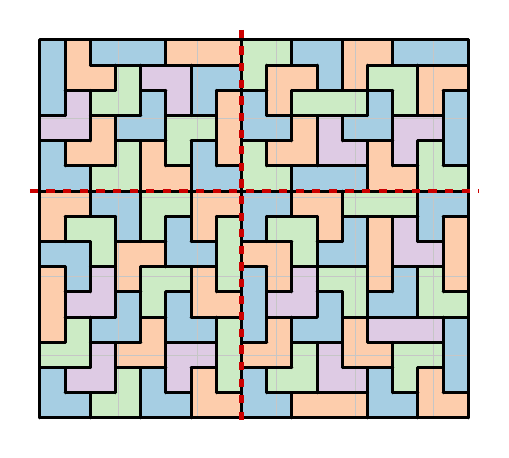
\begin{tikzpicture}[x=0.32cm,y=0.32cm]
\fill[tileA] (0,0) rectangle ++(1,-1);
\fill[tileA] (0,-1) rectangle ++(1,-1);
\fill[tileA] (0,-2) rectangle ++(1,-1);
\fill[tileB] (1,0) rectangle ++(1,-1);
\fill[tileB] (1,-1) rectangle ++(1,-1);
\fill[tileB] (2,-1) rectangle ++(1,-1);
\fill[tileA] (2,0) rectangle ++(1,-1);
\fill[tileA] (3,0) rectangle ++(1,-1);
\fill[tileA] (4,0) rectangle ++(1,-1);
\fill[tileB] (5,0) rectangle ++(1,-1);
\fill[tileB] (6,0) rectangle ++(1,-1);
\fill[tileB] (7,0) rectangle ++(1,-1);
\fill[tileC] (3,-1) rectangle ++(1,-1);
\fill[tileC] (2,-2) rectangle ++(1,-1);
\fill[tileC] (3,-2) rectangle ++(1,-1);
\fill[tileD] (4,-1) rectangle ++(1,-1);
\fill[tileD] (5,-1) rectangle ++(1,-1);
\fill[tileD] (5,-2) rectangle ++(1,-1);
\fill[tileA] (6,-1) rectangle ++(1,-1);
\fill[tileA] (7,-1) rectangle ++(1,-1);
\fill[tileA] (6,-2) rectangle ++(1,-1);
\fill[tileD] (1,-2) rectangle ++(1,-1);
\fill[tileD] (0,-3) rectangle ++(1,-1);
\fill[tileD] (1,-3) rectangle ++(1,-1);
\fill[tileA] (4,-2) rectangle ++(1,-1);
\fill[tileA] (3,-3) rectangle ++(1,-1);
\fill[tileA] (4,-3) rectangle ++(1,-1);
\fill[tileB] (7,-2) rectangle ++(1,-1);
\fill[tileB] (7,-3) rectangle ++(1,-1);
\fill[tileB] (7,-4) rectangle ++(1,-1);
\fill[tileB] (2,-3) rectangle ++(1,-1);
\fill[tileB] (1,-4) rectangle ++(1,-1);
\fill[tileB] (2,-4) rectangle ++(1,-1);
\fill[tileC] (5,-3) rectangle ++(1,-1);
\fill[tileC] (6,-3) rectangle ++(1,-1);
\fill[tileC] (5,-4) rectangle ++(1,-1);
\fill[tileA] (0,-4) rectangle ++(1,-1);
\fill[tileA] (0,-5) rectangle ++(1,-1);
\fill[tileA] (1,-5) rectangle ++(1,-1);
\fill[tileC] (3,-4) rectangle ++(1,-1);
\fill[tileC] (2,-5) rectangle ++(1,-1);
\fill[tileC] (3,-5) rectangle ++(1,-1);
\fill[tileB] (4,-4) rectangle ++(1,-1);
\fill[tileB] (4,-5) rectangle ++(1,-1);
\fill[tileB] (5,-5) rectangle ++(1,-1);
\fill[tileA] (6,-4) rectangle ++(1,-1);
\fill[tileA] (6,-5) rectangle ++(1,-1);
\fill[tileA] (7,-5) rectangle ++(1,-1);
\fill[tileC] (8,0) rectangle ++(1,-1);
\fill[tileC] (9,0) rectangle ++(1,-1);
\fill[tileC] (8,-1) rectangle ++(1,-1);
\fill[tileA] (10,0) rectangle ++(1,-1);
\fill[tileA] (11,0) rectangle ++(1,-1);
\fill[tileA] (11,-1) rectangle ++(1,-1);
\fill[tileB] (12,0) rectangle ++(1,-1);
\fill[tileB] (13,0) rectangle ++(1,-1);
\fill[tileB] (12,-1) rectangle ++(1,-1);
\fill[tileA] (14,0) rectangle ++(1,-1);
\fill[tileA] (15,0) rectangle ++(1,-1);
\fill[tileA] (16,0) rectangle ++(1,-1);
\fill[tileB] (9,-1) rectangle ++(1,-1);
\fill[tileB] (10,-1) rectangle ++(1,-1);
\fill[tileB] (9,-2) rectangle ++(1,-1);
\fill[tileC] (13,-1) rectangle ++(1,-1);
\fill[tileC] (14,-1) rectangle ++(1,-1);
\fill[tileC] (14,-2) rectangle ++(1,-1);
\fill[tileB] (15,-1) rectangle ++(1,-1);
\fill[tileB] (16,-1) rectangle ++(1,-1);
\fill[tileB] (15,-2) rectangle ++(1,-1);
\fill[tileA] (8,-2) rectangle ++(1,-1);
\fill[tileA] (8,-3) rectangle ++(1,-1);
\fill[tileA] (9,-3) rectangle ++(1,-1);
\fill[tileC] (10,-2) rectangle ++(1,-1);
\fill[tileC] (11,-2) rectangle ++(1,-1);
\fill[tileC] (12,-2) rectangle ++(1,-1);
\fill[tileA] (13,-2) rectangle ++(1,-1);
\fill[tileA] (12,-3) rectangle ++(1,-1);
\fill[tileA] (13,-3) rectangle ++(1,-1);
\fill[tileA] (16,-2) rectangle ++(1,-1);
\fill[tileA] (16,-3) rectangle ++(1,-1);
\fill[tileA] (16,-4) rectangle ++(1,-1);
\fill[tileB] (10,-3) rectangle ++(1,-1);
\fill[tileB] (9,-4) rectangle ++(1,-1);
\fill[tileB] (10,-4) rectangle ++(1,-1);
\fill[tileD] (11,-3) rectangle ++(1,-1);
\fill[tileD] (11,-4) rectangle ++(1,-1);
\fill[tileD] (12,-4) rectangle ++(1,-1);
\fill[tileD] (14,-3) rectangle ++(1,-1);
\fill[tileD] (15,-3) rectangle ++(1,-1);
\fill[tileD] (14,-4) rectangle ++(1,-1);
\fill[tileC] (8,-4) rectangle ++(1,-1);
\fill[tileC] (8,-5) rectangle ++(1,-1);
\fill[tileC] (9,-5) rectangle ++(1,-1);
\fill[tileB] (13,-4) rectangle ++(1,-1);
\fill[tileB] (13,-5) rectangle ++(1,-1);
\fill[tileB] (14,-5) rectangle ++(1,-1);
\fill[tileC] (15,-4) rectangle ++(1,-1);
\fill[tileC] (15,-5) rectangle ++(1,-1);
\fill[tileC] (16,-5) rectangle ++(1,-1);
\fill[tileA] (10,-5) rectangle ++(1,-1);
\fill[tileA] (11,-5) rectangle ++(1,-1);
\fill[tileA] (12,-5) rectangle ++(1,-1);
\fill[tileB] (0,-6) rectangle ++(1,-1);
\fill[tileB] (1,-6) rectangle ++(1,-1);
\fill[tileB] (0,-7) rectangle ++(1,-1);
\fill[tileA] (2,-6) rectangle ++(1,-1);
\fill[tileA] (3,-6) rectangle ++(1,-1);
\fill[tileA] (3,-7) rectangle ++(1,-1);
\fill[tileC] (4,-6) rectangle ++(1,-1);
\fill[tileC] (5,-6) rectangle ++(1,-1);
\fill[tileC] (4,-7) rectangle ++(1,-1);
\fill[tileB] (6,-6) rectangle ++(1,-1);
\fill[tileB] (7,-6) rectangle ++(1,-1);
\fill[tileB] (6,-7) rectangle ++(1,-1);
\fill[tileC] (1,-7) rectangle ++(1,-1);
\fill[tileC] (2,-7) rectangle ++(1,-1);
\fill[tileC] (2,-8) rectangle ++(1,-1);
\fill[tileA] (5,-7) rectangle ++(1,-1);
\fill[tileA] (5,-8) rectangle ++(1,-1);
\fill[tileA] (6,-8) rectangle ++(1,-1);
\fill[tileC] (7,-7) rectangle ++(1,-1);
\fill[tileC] (7,-8) rectangle ++(1,-1);
\fill[tileC] (7,-9) rectangle ++(1,-1);
\fill[tileA] (0,-8) rectangle ++(1,-1);
\fill[tileA] (1,-8) rectangle ++(1,-1);
\fill[tileA] (1,-9) rectangle ++(1,-1);
\fill[tileB] (3,-8) rectangle ++(1,-1);
\fill[tileB] (4,-8) rectangle ++(1,-1);
\fill[tileB] (3,-9) rectangle ++(1,-1);
\fill[tileB] (0,-9) rectangle ++(1,-1);
\fill[tileB] (0,-10) rectangle ++(1,-1);
\fill[tileB] (0,-11) rectangle ++(1,-1);
\fill[tileD] (2,-9) rectangle ++(1,-1);
\fill[tileD] (1,-10) rectangle ++(1,-1);
\fill[tileD] (2,-10) rectangle ++(1,-1);
\fill[tileC] (4,-9) rectangle ++(1,-1);
\fill[tileC] (5,-9) rectangle ++(1,-1);
\fill[tileC] (4,-10) rectangle ++(1,-1);
\fill[tileB] (6,-9) rectangle ++(1,-1);
\fill[tileB] (6,-10) rectangle ++(1,-1);
\fill[tileB] (7,-10) rectangle ++(1,-1);
\fill[tileA] (3,-10) rectangle ++(1,-1);
\fill[tileA] (2,-11) rectangle ++(1,-1);
\fill[tileA] (3,-11) rectangle ++(1,-1);
\fill[tileA] (5,-10) rectangle ++(1,-1);
\fill[tileA] (5,-11) rectangle ++(1,-1);
\fill[tileA] (6,-11) rectangle ++(1,-1);
\fill[tileC] (1,-11) rectangle ++(1,-1);
\fill[tileC] (0,-12) rectangle ++(1,-1);
\fill[tileC] (1,-12) rectangle ++(1,-1);
\fill[tileB] (4,-11) rectangle ++(1,-1);
\fill[tileB] (3,-12) rectangle ++(1,-1);
\fill[tileB] (4,-12) rectangle ++(1,-1);
\fill[tileC] (7,-11) rectangle ++(1,-1);
\fill[tileC] (7,-12) rectangle ++(1,-1);
\fill[tileC] (7,-13) rectangle ++(1,-1);
\fill[tileD] (2,-12) rectangle ++(1,-1);
\fill[tileD] (1,-13) rectangle ++(1,-1);
\fill[tileD] (2,-13) rectangle ++(1,-1);
\fill[tileD] (5,-12) rectangle ++(1,-1);
\fill[tileD] (6,-12) rectangle ++(1,-1);
\fill[tileD] (5,-13) rectangle ++(1,-1);
\fill[tileA] (0,-13) rectangle ++(1,-1);
\fill[tileA] (0,-14) rectangle ++(1,-1);
\fill[tileA] (1,-14) rectangle ++(1,-1);
\fill[tileC] (3,-13) rectangle ++(1,-1);
\fill[tileC] (2,-14) rectangle ++(1,-1);
\fill[tileC] (3,-14) rectangle ++(1,-1);
\fill[tileA] (4,-13) rectangle ++(1,-1);
\fill[tileA] (4,-14) rectangle ++(1,-1);
\fill[tileA] (5,-14) rectangle ++(1,-1);
\fill[tileB] (6,-13) rectangle ++(1,-1);
\fill[tileB] (6,-14) rectangle ++(1,-1);
\fill[tileB] (7,-14) rectangle ++(1,-1);
\fill[tileA] (8,-6) rectangle ++(1,-1);
\fill[tileA] (9,-6) rectangle ++(1,-1);
\fill[tileA] (8,-7) rectangle ++(1,-1);
\fill[tileB] (10,-6) rectangle ++(1,-1);
\fill[tileB] (11,-6) rectangle ++(1,-1);
\fill[tileB] (11,-7) rectangle ++(1,-1);
\fill[tileC] (12,-6) rectangle ++(1,-1);
\fill[tileC] (13,-6) rectangle ++(1,-1);
\fill[tileC] (14,-6) rectangle ++(1,-1);
\fill[tileA] (15,-6) rectangle ++(1,-1);
\fill[tileA] (16,-6) rectangle ++(1,-1);
\fill[tileA] (15,-7) rectangle ++(1,-1);
\fill[tileC] (9,-7) rectangle ++(1,-1);
\fill[tileC] (10,-7) rectangle ++(1,-1);
\fill[tileC] (10,-8) rectangle ++(1,-1);
\fill[tileA] (12,-7) rectangle ++(1,-1);
\fill[tileA] (11,-8) rectangle ++(1,-1);
\fill[tileA] (12,-8) rectangle ++(1,-1);
\fill[tileB] (13,-7) rectangle ++(1,-1);
\fill[tileB] (13,-8) rectangle ++(1,-1);
\fill[tileB] (13,-9) rectangle ++(1,-1);
\fill[tileD] (14,-7) rectangle ++(1,-1);
\fill[tileD] (14,-8) rectangle ++(1,-1);
\fill[tileD] (15,-8) rectangle ++(1,-1);
\fill[tileB] (16,-7) rectangle ++(1,-1);
\fill[tileB] (16,-8) rectangle ++(1,-1);
\fill[tileB] (16,-9) rectangle ++(1,-1);
\fill[tileB] (8,-8) rectangle ++(1,-1);
\fill[tileB] (9,-8) rectangle ++(1,-1);
\fill[tileB] (9,-9) rectangle ++(1,-1);
\fill[tileA] (8,-9) rectangle ++(1,-1);
\fill[tileA] (8,-10) rectangle ++(1,-1);
\fill[tileA] (8,-11) rectangle ++(1,-1);
\fill[tileD] (10,-9) rectangle ++(1,-1);
\fill[tileD] (9,-10) rectangle ++(1,-1);
\fill[tileD] (10,-10) rectangle ++(1,-1);
\fill[tileC] (11,-9) rectangle ++(1,-1);
\fill[tileC] (12,-9) rectangle ++(1,-1);
\fill[tileC] (12,-10) rectangle ++(1,-1);
\fill[tileA] (14,-9) rectangle ++(1,-1);
\fill[tileA] (13,-10) rectangle ++(1,-1);
\fill[tileA] (14,-10) rectangle ++(1,-1);
\fill[tileC] (15,-9) rectangle ++(1,-1);
\fill[tileC] (15,-10) rectangle ++(1,-1);
\fill[tileC] (16,-10) rectangle ++(1,-1);
\fill[tileA] (11,-10) rectangle ++(1,-1);
\fill[tileA] (10,-11) rectangle ++(1,-1);
\fill[tileA] (11,-11) rectangle ++(1,-1);
\fill[tileB] (9,-11) rectangle ++(1,-1);
\fill[tileB] (8,-12) rectangle ++(1,-1);
\fill[tileB] (9,-12) rectangle ++(1,-1);
\fill[tileB] (12,-11) rectangle ++(1,-1);
\fill[tileB] (12,-12) rectangle ++(1,-1);
\fill[tileB] (13,-12) rectangle ++(1,-1);
\fill[tileD] (13,-11) rectangle ++(1,-1);
\fill[tileD] (14,-11) rectangle ++(1,-1);
\fill[tileD] (15,-11) rectangle ++(1,-1);
\fill[tileA] (16,-11) rectangle ++(1,-1);
\fill[tileA] (16,-12) rectangle ++(1,-1);
\fill[tileA] (16,-13) rectangle ++(1,-1);
\fill[tileC] (10,-12) rectangle ++(1,-1);
\fill[tileC] (9,-13) rectangle ++(1,-1);
\fill[tileC] (10,-13) rectangle ++(1,-1);
\fill[tileD] (11,-12) rectangle ++(1,-1);
\fill[tileD] (11,-13) rectangle ++(1,-1);
\fill[tileD] (12,-13) rectangle ++(1,-1);
\fill[tileC] (14,-12) rectangle ++(1,-1);
\fill[tileC] (15,-12) rectangle ++(1,-1);
\fill[tileC] (14,-13) rectangle ++(1,-1);
\fill[tileA] (8,-13) rectangle ++(1,-1);
\fill[tileA] (8,-14) rectangle ++(1,-1);
\fill[tileA] (9,-14) rectangle ++(1,-1);
\fill[tileA] (13,-13) rectangle ++(1,-1);
\fill[tileA] (13,-14) rectangle ++(1,-1);
\fill[tileA] (14,-14) rectangle ++(1,-1);
\fill[tileB] (15,-13) rectangle ++(1,-1);
\fill[tileB] (15,-14) rectangle ++(1,-1);
\fill[tileB] (16,-14) rectangle ++(1,-1);
\fill[tileB] (10,-14) rectangle ++(1,-1);
\fill[tileB] (11,-14) rectangle ++(1,-1);
\fill[tileB] (12,-14) rectangle ++(1,-1);
\draw[cellgrid] (0,0) grid (17,-15);
\draw[tileedge] (1,0)--++(0,-1) (2,0)--++(0,-1) (2,-1)--++(1,0) (3,-1)--++(1,0) (5,0)--++(0,-1) (4,-1)--++(1,0) (5,-1)--++(1,0) (6,-1)--++(1,0);
\draw[tileedge] (8,0)--++(0,-1) (7,-1)--++(1,0) (10,0)--++(0,-1) (9,-1)--++(1,0) (10,-1)--++(1,0) (12,0)--++(0,-1) (14,0)--++(0,-1) (13,-1)--++(1,0);
\draw[tileedge] (14,-1)--++(1,0) (15,-1)--++(1,0) (17,0)--++(0,-1) (16,-1)--++(1,0) (1,-1)--++(0,-1) (1,-2)--++(1,0) (3,-1)--++(0,-1) (2,-2)--++(1,0);
\draw[tileedge] (4,-1)--++(0,-1) (4,-2)--++(1,0) (6,-1)--++(0,-1) (8,-1)--++(0,-1) (7,-2)--++(1,0) (9,-1)--++(0,-1) (8,-2)--++(1,0) (11,-1)--++(0,-1);
\draw[tileedge] (10,-2)--++(1,0) (12,-1)--++(0,-1) (11,-2)--++(1,0) (13,-1)--++(0,-1) (12,-2)--++(1,0) (13,-2)--++(1,0) (15,-1)--++(0,-1) (17,-1)--++(0,-1);
\draw[tileedge] (16,-2)--++(1,0) (1,-2)--++(0,-1) (0,-3)--++(1,0) (2,-2)--++(0,-1) (2,-3)--++(1,0) (4,-2)--++(0,-1) (3,-3)--++(1,0) (5,-2)--++(0,-1);
\draw[tileedge] (6,-2)--++(0,-1) (5,-3)--++(1,0) (7,-2)--++(0,-1) (6,-3)--++(1,0) (8,-2)--++(0,-1) (9,-2)--++(0,-1) (10,-2)--++(0,-1) (9,-3)--++(1,0);
\draw[tileedge] (10,-3)--++(1,0) (11,-3)--++(1,0) (13,-2)--++(0,-1) (12,-3)--++(1,0) (14,-2)--++(0,-1) (15,-2)--++(0,-1) (14,-3)--++(1,0) (16,-2)--++(0,-1);
\draw[tileedge] (15,-3)--++(1,0) (17,-2)--++(0,-1) (0,-4)--++(1,0) (2,-3)--++(0,-1) (1,-4)--++(1,0) (3,-3)--++(0,-1) (3,-4)--++(1,0) (5,-3)--++(0,-1);
\draw[tileedge] (4,-4)--++(1,0) (7,-3)--++(0,-1) (6,-4)--++(1,0) (8,-3)--++(0,-1) (8,-4)--++(1,0) (10,-3)--++(0,-1) (9,-4)--++(1,0) (11,-3)--++(0,-1);
\draw[tileedge] (12,-3)--++(0,-1) (12,-4)--++(1,0) (14,-3)--++(0,-1) (13,-4)--++(1,0) (16,-3)--++(0,-1) (15,-4)--++(1,0) (17,-3)--++(0,-1) (1,-4)--++(0,-1);
\draw[tileedge] (1,-5)--++(1,0) (3,-4)--++(0,-1) (2,-5)--++(1,0) (4,-4)--++(0,-1) (5,-4)--++(0,-1) (6,-4)--++(0,-1) (5,-5)--++(1,0) (7,-4)--++(0,-1);
\draw[tileedge] (8,-4)--++(0,-1) (7,-5)--++(1,0) (9,-4)--++(0,-1) (9,-5)--++(1,0) (11,-4)--++(0,-1) (10,-5)--++(1,0) (11,-5)--++(1,0) (13,-4)--++(0,-1);
\draw[tileedge] (12,-5)--++(1,0) (14,-4)--++(0,-1) (15,-4)--++(0,-1) (14,-5)--++(1,0) (16,-4)--++(0,-1) (17,-4)--++(0,-1) (16,-5)--++(1,0) (0,-6)--++(1,0);
\draw[tileedge] (2,-5)--++(0,-1) (1,-6)--++(1,0) (2,-6)--++(1,0) (4,-5)--++(0,-1) (3,-6)--++(1,0) (4,-6)--++(1,0) (6,-5)--++(0,-1) (5,-6)--++(1,0);
\draw[tileedge] (6,-6)--++(1,0) (8,-5)--++(0,-1) (7,-6)--++(1,0) (8,-6)--++(1,0) (10,-5)--++(0,-1) (9,-6)--++(1,0) (10,-6)--++(1,0) (11,-6)--++(1,0);
\draw[tileedge] (13,-5)--++(0,-1) (12,-6)--++(1,0) (13,-6)--++(1,0) (15,-5)--++(0,-1) (14,-6)--++(1,0) (15,-6)--++(1,0) (17,-5)--++(0,-1) (16,-6)--++(1,0);
\draw[tileedge] (2,-6)--++(0,-1) (1,-7)--++(1,0) (2,-7)--++(1,0) (4,-6)--++(0,-1) (6,-6)--++(0,-1) (5,-7)--++(1,0) (8,-6)--++(0,-1) (7,-7)--++(1,0);
\draw[tileedge] (10,-6)--++(0,-1) (9,-7)--++(1,0) (10,-7)--++(1,0) (12,-6)--++(0,-1) (12,-7)--++(1,0) (13,-7)--++(1,0) (15,-6)--++(0,-1) (14,-7)--++(1,0);
\draw[tileedge] (17,-6)--++(0,-1) (16,-7)--++(1,0) (1,-7)--++(0,-1) (0,-8)--++(1,0) (1,-8)--++(1,0) (3,-7)--++(0,-1) (4,-7)--++(0,-1) (3,-8)--++(1,0);
\draw[tileedge] (5,-7)--++(0,-1) (4,-8)--++(1,0) (6,-7)--++(0,-1) (7,-7)--++(0,-1) (6,-8)--++(1,0) (8,-7)--++(0,-1) (9,-7)--++(0,-1) (8,-8)--++(1,0);
\draw[tileedge] (9,-8)--++(1,0) (11,-7)--++(0,-1) (12,-7)--++(0,-1) (11,-8)--++(1,0) (13,-7)--++(0,-1) (14,-7)--++(0,-1) (15,-7)--++(0,-1) (16,-7)--++(0,-1);
\draw[tileedge] (15,-8)--++(1,0) (17,-7)--++(0,-1) (0,-9)--++(1,0) (2,-8)--++(0,-1) (3,-8)--++(0,-1) (2,-9)--++(1,0) (5,-8)--++(0,-1) (4,-9)--++(1,0);
\draw[tileedge] (5,-9)--++(1,0) (7,-8)--++(0,-1) (6,-9)--++(1,0) (8,-8)--++(0,-1) (8,-9)--++(1,0) (10,-8)--++(0,-1) (11,-8)--++(0,-1) (10,-9)--++(1,0);
\draw[tileedge] (11,-9)--++(1,0) (13,-8)--++(0,-1) (12,-9)--++(1,0) (14,-8)--++(0,-1) (14,-9)--++(1,0) (16,-8)--++(0,-1) (15,-9)--++(1,0) (17,-8)--++(0,-1);
\draw[tileedge] (1,-9)--++(0,-1) (2,-9)--++(0,-1) (1,-10)--++(1,0) (3,-9)--++(0,-1) (4,-9)--++(0,-1) (3,-10)--++(1,0) (6,-9)--++(0,-1) (5,-10)--++(1,0);
\draw[tileedge] (7,-9)--++(0,-1) (8,-9)--++(0,-1) (7,-10)--++(1,0) (9,-9)--++(0,-1) (10,-9)--++(0,-1) (9,-10)--++(1,0) (11,-9)--++(0,-1) (11,-10)--++(1,0);
\draw[tileedge] (13,-9)--++(0,-1) (14,-9)--++(0,-1) (13,-10)--++(1,0) (15,-9)--++(0,-1) (16,-9)--++(0,-1) (17,-9)--++(0,-1) (16,-10)--++(1,0) (1,-10)--++(0,-1);
\draw[tileedge] (1,-11)--++(1,0) (3,-10)--++(0,-1) (2,-11)--++(1,0) (4,-10)--++(0,-1) (5,-10)--++(0,-1) (4,-11)--++(1,0) (6,-10)--++(0,-1) (6,-11)--++(1,0);
\draw[tileedge] (8,-10)--++(0,-1) (7,-11)--++(1,0) (9,-10)--++(0,-1) (9,-11)--++(1,0) (11,-10)--++(0,-1) (10,-11)--++(1,0) (12,-10)--++(0,-1) (13,-10)--++(0,-1);
\draw[tileedge] (12,-11)--++(1,0) (13,-11)--++(1,0) (15,-10)--++(0,-1) (14,-11)--++(1,0) (15,-11)--++(1,0) (17,-10)--++(0,-1) (16,-11)--++(1,0) (1,-11)--++(0,-1);
\draw[tileedge] (0,-12)--++(1,0) (2,-11)--++(0,-1) (2,-12)--++(1,0) (4,-11)--++(0,-1) (3,-12)--++(1,0) (5,-11)--++(0,-1) (5,-12)--++(1,0) (7,-11)--++(0,-1);
\draw[tileedge] (6,-12)--++(1,0) (8,-11)--++(0,-1) (9,-11)--++(0,-1) (8,-12)--++(1,0) (10,-11)--++(0,-1) (10,-12)--++(1,0) (12,-11)--++(0,-1) (11,-12)--++(1,0);
\draw[tileedge] (13,-11)--++(0,-1) (13,-12)--++(1,0) (14,-12)--++(1,0) (16,-11)--++(0,-1) (15,-12)--++(1,0) (17,-11)--++(0,-1) (0,-13)--++(1,0) (2,-12)--++(0,-1);
\draw[tileedge] (1,-13)--++(1,0) (3,-12)--++(0,-1) (3,-13)--++(1,0) (5,-12)--++(0,-1) (4,-13)--++(1,0) (7,-12)--++(0,-1) (6,-13)--++(1,0) (8,-12)--++(0,-1);
\draw[tileedge] (8,-13)--++(1,0) (10,-12)--++(0,-1) (9,-13)--++(1,0) (11,-12)--++(0,-1) (12,-12)--++(0,-1) (12,-13)--++(1,0) (14,-12)--++(0,-1) (13,-13)--++(1,0);
\draw[tileedge] (16,-12)--++(0,-1) (15,-13)--++(1,0) (17,-12)--++(0,-1) (1,-13)--++(0,-1) (1,-14)--++(1,0) (3,-13)--++(0,-1) (2,-14)--++(1,0) (4,-13)--++(0,-1);
\draw[tileedge] (5,-13)--++(0,-1) (6,-13)--++(0,-1) (5,-14)--++(1,0) (7,-13)--++(0,-1) (8,-13)--++(0,-1) (7,-14)--++(1,0) (9,-13)--++(0,-1) (9,-14)--++(1,0);
\draw[tileedge] (11,-13)--++(0,-1) (10,-14)--++(1,0) (11,-14)--++(1,0) (13,-13)--++(0,-1) (12,-14)--++(1,0) (14,-13)--++(0,-1) (15,-13)--++(0,-1) (14,-14)--++(1,0);
\draw[tileedge] (16,-13)--++(0,-1) (17,-13)--++(0,-1) (16,-14)--++(1,0) (0,-15)--++(1,0) (2,-14)--++(0,-1) (1,-15)--++(1,0) (2,-15)--++(1,0) (4,-14)--++(0,-1);
\draw[tileedge] (3,-15)--++(1,0) (4,-15)--++(1,0) (6,-14)--++(0,-1) (5,-15)--++(1,0) (6,-15)--++(1,0) (8,-14)--++(0,-1) (7,-15)--++(1,0) (8,-15)--++(1,0);
\draw[tileedge] (10,-14)--++(0,-1) (9,-15)--++(1,0) (10,-15)--++(1,0) (11,-15)--++(1,0) (13,-14)--++(0,-1) (12,-15)--++(1,0) (13,-15)--++(1,0) (15,-14)--++(0,-1);
\draw[tileedge] (14,-15)--++(1,0) (15,-15)--++(1,0) (17,-14)--++(0,-1) (16,-15)--++(1,0) (0,0)--++(0,-1) (0,-1)--++(0,-1) (0,-2)--++(0,-1) (0,-3)--++(0,-1);
\draw[tileedge] (0,-4)--++(0,-1) (0,-5)--++(0,-1) (0,-6)--++(0,-1) (0,-7)--++(0,-1) (0,-8)--++(0,-1) (0,-9)--++(0,-1) (0,-10)--++(0,-1) (0,-11)--++(0,-1);
\draw[tileedge] (0,-12)--++(0,-1) (0,-13)--++(0,-1) (0,-14)--++(0,-1) (0,0)--++(1,0) (1,0)--++(1,0) (2,0)--++(1,0) (3,0)--++(1,0) (4,0)--++(1,0);
\draw[tileedge] (5,0)--++(1,0) (6,0)--++(1,0) (7,0)--++(1,0) (8,0)--++(1,0) (9,0)--++(1,0) (10,0)--++(1,0) (11,0)--++(1,0) (12,0)--++(1,0);
\draw[tileedge] (13,0)--++(1,0) (14,0)--++(1,0) (15,0)--++(1,0) (16,0)--++(1,0);
\draw[seam] (-0.4,-6)--(17.4,-6);
\draw[seam] (8,0.4)--(8,-15.4);
\end{tikzpicture}
%% END FIGURE palette
\caption{The four blocks for widths $n\ge56$, of heights 6 and 9 and widths
8 and 9, here in a $15\times17$ rectangle with the horizontal and vertical
seams dashed. Each block also stacks on and fits beside every block of the
same width or height, including itself, so these four fill every
rectangle with $3\mid m$, $m\ge6$ and $n\ge56$.}
\label{fig:palette}
\end{figure}

\begin{lemma}\label{lem:arith}
\begin{enumerate}
\item[(a)] Every multiple of 3 that is at least 6 is $6a+9b$ for some
integers $a,b\ge0$.
\item[(b)] Every integer that is at least 56 is $8a+9b$ for some integers
$a,b\ge0$.
\item[(c)] Every multiple of 3 that is at least 9, other than 15, is
$9a+12b$ for some integers $a,b\ge0$.
\end{enumerate}
\end{lemma}

\begin{proof}
(a) Write $m=3q$ with $q\ge2$. If $q$ is even, $m=6\cdot(q/2)$; if $q$ is
odd, then $q\ge3$ and $m=9+6\cdot(q-3)/2$. (b) Write $n=8Q+r$ with
$0\le r\le7$. Then $Q\ge7\ge r$ and $n=8(Q-r)+9r$. (c) Dividing by 3, we
need every integer $q\ge3$ other than 5 to be $3a+4b$: this holds for
$q=3,4,6,7,8$, and adding threes reaches every larger integer.
\end{proof}

\begin{proof}[Proof of Theorem~\ref{thm:conj}]
Let $3\mid m$, $m\ge6$ and $n\ge4$. By Lemma~\ref{lem:two} it suffices to
find a tiling of the $m\times n$ rectangle all of whose pairs of tiles are
rigid.

If $n\ge56$, Lemma~\ref{lem:arith}(a),(b) writes $m$ as a sum of sixes and
nines and $n$ as a sum of eights and nines, and Corollary~\ref{cor:assemble}(ii)
with the blocks of Proposition~\ref{prop:blocks}(iii) gives the tiling.

If $4\le n\le55$ and $n\ne5$, Lemma~\ref{lem:arith}(a) writes $m$ as a sum
of sixes and nines, and Corollary~\ref{cor:assemble}(i) with the blocks
$B_{6,n}$ and $B_{9,n}$ of Proposition~\ref{prop:blocks}(i) gives the tiling.

If $n=5$ and $m\in\{6,15\}$, Proposition~\ref{prop:blocks}(ii) gives the
tiling directly. Otherwise $m\ge9$ and $m\ne15$, Lemma~\ref{lem:arith}(c)
writes $m$ as a sum of nines and twelves, and Corollary~\ref{cor:assemble}(i)
with $B_{9,5}$ and $B_{12,5}$ gives the tiling.
\end{proof}


\section{Proof of the classification}\label{sec:main}

\begin{proof}[Proof of Theorem~\ref{thm:main}]
Suppose first that the $m\times n$ rectangle has a locked tiling $T$. Its
$mn$ cells are split into tiles of three cells, so $3\mid mn$. Suppose that
$\min(m,n)\le3$. Transposing if necessary, we may assume $m\le3$; then
$M(G(m,n),3)$ is connected by Theorem~\ref{thm:narrow}. But $T$ is an
isolated vertex of this graph, and the graph has another vertex, so it is not
connected. This contradiction shows $\min(m,n)\ge4$.

Conversely, suppose $3\mid mn$ and $\min(m,n)\ge4$. Since 3 is prime, it
divides $m$ or $n$; transposing if necessary, $3\mid m$. As $m\ge4$ and $m$
is a multiple of 3, $m\ge6$. Also $n\ge4$, so Theorem~\ref{thm:conj} gives a
locked tiling of the $m\times n$ rectangle, and transposing back gives one of
the original rectangle.
\end{proof}

\section{Formal verification}\label{sec:formal}

The formal theorem is
\file{LockedTromino.Witnesses.locked_tromino_rectangles}:
\[
\forall\, m\ n,\quad 6\le m \;\to\; 3\mid m \;\to\; 4\le n \;\to\;
\exists\, T,\ \mathrm{Locked}\,(\mathrm{Rectangle}\ m\ n)\ T.
\]
Here $m,n$ are natural numbers. The formal definitions use integer-pair
cells and adjacency through shared sides. The rectangle consists of
$0\le i<m$, $0\le j<n$; a tile is a connected set of three distinct
cells, a tiling is a partition into such sets, and rigidity means that every
split of two tiles into two trominoes gives the original unordered pair.
The predicate $\mathrm{Locked}$ combines this partition and pairwise
rigidity with the existence of a different tiling, exactly as in
Section~\ref{sec:defs}. Thus the
statement is Theorem~\ref{thm:conj}, whose hypotheses make its integer
parameters natural numbers, with no additional assumptions. The proof
formalizes Lemmas~\ref{lem:apart}, \ref{lem:two}, \ref{lem:glue}
and~\ref{lem:arith}, Corollary~\ref{cor:assemble} and
Proposition~\ref{prop:blocks}. Theorem~\ref{thm:main} additionally uses the
written deduction in Section~\ref{sec:main} and Tucker-Foltz's
Theorem~3.1, which remains outside Lean.

Lean's kernel checks the finite assertions by reduction, using
\texttt{decide} and \texttt{rfl}, without \texttt{native\_decide} or
\texttt{Lean.ofReduceBool}. The main existence theorem depends on exactly
\texttt{propext}, \texttt{Classical.choice} and \texttt{Quot.sound}. Two separately
written programs, sharing no code, independently enumerate all partitions
of each six-cell union into two trominoes. The small-count comparison is
in Appendix~\ref{app:checks}. Checking notes supplied with the paper give
the logical axioms, reproduction commands and resource estimates.

\section*{Acknowledgments}
Jamie Tucker-Foltz posed the problem, gave the definitions used here, proved
the case of narrow grids and the case $n\ge100$ by the block method we
follow, and computed the small cases used to check our enumeration. Lean and its
contributors supplied the formal-proof system.


\clearpage
\begin{appendices}
\section{The blocks}\label{app:data}

This appendix describes where the tilings of Proposition~\ref{prop:blocks}
are: their coordinates are in the folder \file{data/} released with this
paper, one JSON file per family, and Figures~\ref{fig:example},
\ref{fig:stack}, \ref{fig:palette} and~\ref{fig:five} draw ten of them. Each file names
its blocks, gives each block's height, width and tiles (each tile a list of
three cells $(i,j)$ with $i$ the row), and lists the seams to be checked:
\texttt{vertical} $[X,Y]$ means $X$ stacks on $Y$, and \texttt{horizontal}
$[X,Y]$ means $X$ fits left of $Y$.

\begin{center}
\begin{tabular}{@{}llrrr@{}}
\toprule
File in \file{data/} & Contents & Blocks & Stacks & Side by side\\
\midrule
\file{witnesses/width-w.json} ($w\ne5$) & $B_{6,w}$, $B_{9,w}$, $4\le w\le55$ & 2 each & 4 each & --\\
\file{witnesses/width-5.json} & $B_{9,5}$, $B_{12,5}$ & 2 & 4 & --\\
\file{witnesses/direct-6x5.json} & a rigid $6\times5$ tiling & 1 & -- & --\\
\file{witnesses/direct-15x5.json} & a rigid $15\times5$ tiling & 1 & -- & --\\
\file{palette.json} & $P_{h,w}$, $h\in\{6,9\}$, $w\in\{8,9\}$ & 4 & 8 & 8\\
\midrule
Total, 55 files & & 110 & 216 & 8\\
\bottomrule
\end{tabular}
\end{center}

In all, the proof uses 110 blocks and 224 ordered seams. The seams of each
family include both orders of two different blocks and each block against a
copy of itself.


\section{Finite checks}\label{app:checks}

The enumeration finds 26 locked tilings of the $6\times4$ rectangle, a
count obtained here. Their 7 symmetry classes and the 50 locked tilings of
the $6\times6$ rectangle agree with Tucker-Foltz's reported counts
\cite[Figure~2 and Section~3]{tf}.

For the finite rigidity checks, only touching pairs need be considered by
Lemma~\ref{lem:apart}. The touching pairs occurring in the blocks and seams fall into 162 shapes up to translation and
order. Each shape is checked once, then reused by translation invariance.
The checking notes describe the cell lists, the complete neighbor lists,
the two separately written programs and their checks on incorrect data.

\section{Additional illustrations}\label{app:figures}

Figure~\ref{fig:move} illustrates a recombination move, Figure~\ref{fig:two}
the two straight tilings of Lemma~\ref{lem:two}, and Figure~\ref{fig:five}
the width-5 constructions of Proposition~\ref{prop:blocks}(ii).

\begin{figure}[ht]
\centering
%% BEGIN FIGURE move
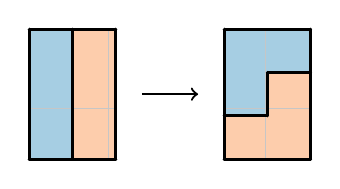
\begin{tikzpicture}[x=0.55cm,y=0.55cm]
\fill[tileA] (0,0) rectangle ++(1,-1);
\fill[tileA] (0,-1) rectangle ++(1,-1);
\fill[tileA] (0,-2) rectangle ++(1,-1);
\fill[tileB] (1,0) rectangle ++(1,-1);
\fill[tileB] (1,-1) rectangle ++(1,-1);
\fill[tileB] (1,-2) rectangle ++(1,-1);
\draw[cellgrid] (0,0) grid (2,-3);
\draw[tileedge] (1,0)--++(0,-1) (2,0)--++(0,-1) (1,-1)--++(0,-1) (2,-1)--++(0,-1) (1,-2)--++(0,-1) (0,-3)--++(1,0) (2,-2)--++(0,-1) (1,-3)--++(1,0);
\draw[tileedge] (0,0)--++(0,-1) (0,-1)--++(0,-1) (0,-2)--++(0,-1) (0,0)--++(1,0) (1,0)--++(1,0);
\draw[->,thick] (2.6,-1.5)--(3.9,-1.5);
\fill[tileA] (4.5,0) rectangle ++(1,-1);
\fill[tileA] (5.5,0) rectangle ++(1,-1);
\fill[tileA] (4.5,-1) rectangle ++(1,-1);
\fill[tileB] (5.5,-1) rectangle ++(1,-1);
\fill[tileB] (4.5,-2) rectangle ++(1,-1);
\fill[tileB] (5.5,-2) rectangle ++(1,-1);
\draw[cellgrid] (4.5,0) grid (6.5,-3);
\draw[tileedge] (6.5,0)--++(0,-1) (5.5,-1)--++(1,0) (5.5,-1)--++(0,-1) (4.5,-2)--++(1,0) (6.5,-1)--++(0,-1) (4.5,-3)--++(1,0) (6.5,-2)--++(0,-1) (5.5,-3)--++(1,0);
\draw[tileedge] (4.5,0)--++(0,-1) (4.5,-1)--++(0,-1) (4.5,-2)--++(0,-1) (4.5,0)--++(1,0) (5.5,0)--++(1,0);
\end{tikzpicture}
%% END FIGURE move
\caption{A recombination move: two straight trominoes side by side cover
the same six cells as two L-trominoes. A locked tiling has no pair of tiles
that allows such a move.}
\label{fig:move}
\end{figure}

\begin{figure}[ht]
\centering
%% BEGIN FIGURE two-tilings
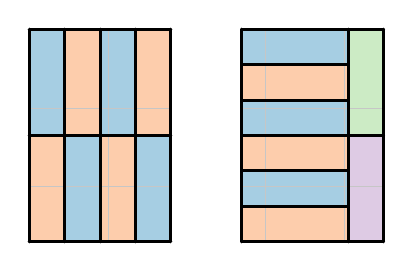
\begin{tikzpicture}[x=0.45cm,y=0.45cm]
\fill[tileA] (0,0) rectangle ++(1,-1);
\fill[tileA] (0,-1) rectangle ++(1,-1);
\fill[tileA] (0,-2) rectangle ++(1,-1);
\fill[tileB] (1,0) rectangle ++(1,-1);
\fill[tileB] (1,-1) rectangle ++(1,-1);
\fill[tileB] (1,-2) rectangle ++(1,-1);
\fill[tileA] (2,0) rectangle ++(1,-1);
\fill[tileA] (2,-1) rectangle ++(1,-1);
\fill[tileA] (2,-2) rectangle ++(1,-1);
\fill[tileB] (3,0) rectangle ++(1,-1);
\fill[tileB] (3,-1) rectangle ++(1,-1);
\fill[tileB] (3,-2) rectangle ++(1,-1);
\fill[tileB] (0,-3) rectangle ++(1,-1);
\fill[tileB] (0,-4) rectangle ++(1,-1);
\fill[tileB] (0,-5) rectangle ++(1,-1);
\fill[tileA] (1,-3) rectangle ++(1,-1);
\fill[tileA] (1,-4) rectangle ++(1,-1);
\fill[tileA] (1,-5) rectangle ++(1,-1);
\fill[tileB] (2,-3) rectangle ++(1,-1);
\fill[tileB] (2,-4) rectangle ++(1,-1);
\fill[tileB] (2,-5) rectangle ++(1,-1);
\fill[tileA] (3,-3) rectangle ++(1,-1);
\fill[tileA] (3,-4) rectangle ++(1,-1);
\fill[tileA] (3,-5) rectangle ++(1,-1);
\draw[cellgrid] (0,0) grid (4,-6);
\draw[tileedge] (1,0)--++(0,-1) (2,0)--++(0,-1) (3,0)--++(0,-1) (4,0)--++(0,-1) (1,-1)--++(0,-1) (2,-1)--++(0,-1) (3,-1)--++(0,-1) (4,-1)--++(0,-1);
\draw[tileedge] (1,-2)--++(0,-1) (0,-3)--++(1,0) (2,-2)--++(0,-1) (1,-3)--++(1,0) (3,-2)--++(0,-1) (2,-3)--++(1,0) (4,-2)--++(0,-1) (3,-3)--++(1,0);
\draw[tileedge] (1,-3)--++(0,-1) (2,-3)--++(0,-1) (3,-3)--++(0,-1) (4,-3)--++(0,-1) (1,-4)--++(0,-1) (2,-4)--++(0,-1) (3,-4)--++(0,-1) (4,-4)--++(0,-1);
\draw[tileedge] (1,-5)--++(0,-1) (0,-6)--++(1,0) (2,-5)--++(0,-1) (1,-6)--++(1,0) (3,-5)--++(0,-1) (2,-6)--++(1,0) (4,-5)--++(0,-1) (3,-6)--++(1,0);
\draw[tileedge] (0,0)--++(0,-1) (0,-1)--++(0,-1) (0,-2)--++(0,-1) (0,-3)--++(0,-1) (0,-4)--++(0,-1) (0,-5)--++(0,-1) (0,0)--++(1,0) (1,0)--++(1,0);
\draw[tileedge] (2,0)--++(1,0) (3,0)--++(1,0);
\fill[tileA] (6,0) rectangle ++(1,-1);
\fill[tileA] (7,0) rectangle ++(1,-1);
\fill[tileA] (8,0) rectangle ++(1,-1);
\fill[tileB] (6,-1) rectangle ++(1,-1);
\fill[tileB] (7,-1) rectangle ++(1,-1);
\fill[tileB] (8,-1) rectangle ++(1,-1);
\fill[tileA] (6,-2) rectangle ++(1,-1);
\fill[tileA] (7,-2) rectangle ++(1,-1);
\fill[tileA] (8,-2) rectangle ++(1,-1);
\fill[tileB] (6,-3) rectangle ++(1,-1);
\fill[tileB] (7,-3) rectangle ++(1,-1);
\fill[tileB] (8,-3) rectangle ++(1,-1);
\fill[tileA] (6,-4) rectangle ++(1,-1);
\fill[tileA] (7,-4) rectangle ++(1,-1);
\fill[tileA] (8,-4) rectangle ++(1,-1);
\fill[tileB] (6,-5) rectangle ++(1,-1);
\fill[tileB] (7,-5) rectangle ++(1,-1);
\fill[tileB] (8,-5) rectangle ++(1,-1);
\fill[tileC] (9,0) rectangle ++(1,-1);
\fill[tileC] (9,-1) rectangle ++(1,-1);
\fill[tileC] (9,-2) rectangle ++(1,-1);
\fill[tileD] (9,-3) rectangle ++(1,-1);
\fill[tileD] (9,-4) rectangle ++(1,-1);
\fill[tileD] (9,-5) rectangle ++(1,-1);
\draw[cellgrid] (6,0) grid (10,-6);
\draw[tileedge] (6,-1)--++(1,0) (7,-1)--++(1,0) (9,0)--++(0,-1) (8,-1)--++(1,0) (10,0)--++(0,-1) (6,-2)--++(1,0) (7,-2)--++(1,0) (9,-1)--++(0,-1);
\draw[tileedge] (8,-2)--++(1,0) (10,-1)--++(0,-1) (6,-3)--++(1,0) (7,-3)--++(1,0) (9,-2)--++(0,-1) (8,-3)--++(1,0) (10,-2)--++(0,-1) (9,-3)--++(1,0);
\draw[tileedge] (6,-4)--++(1,0) (7,-4)--++(1,0) (9,-3)--++(0,-1) (8,-4)--++(1,0) (10,-3)--++(0,-1) (6,-5)--++(1,0) (7,-5)--++(1,0) (9,-4)--++(0,-1);
\draw[tileedge] (8,-5)--++(1,0) (10,-4)--++(0,-1) (6,-6)--++(1,0) (7,-6)--++(1,0) (9,-5)--++(0,-1) (8,-6)--++(1,0) (10,-5)--++(0,-1) (9,-6)--++(1,0);
\draw[tileedge] (6,0)--++(0,-1) (6,-1)--++(0,-1) (6,-2)--++(0,-1) (6,-3)--++(0,-1) (6,-4)--++(0,-1) (6,-5)--++(0,-1) (6,0)--++(1,0) (7,0)--++(1,0);
\draw[tileedge] (8,0)--++(1,0) (9,0)--++(1,0);
\end{tikzpicture}
%% END FIGURE two-tilings
\caption{Two tilings of the $6\times4$ rectangle (Lemma~\ref{lem:two}). Every
rectangle with $3\mid m$ and $n\ge3$ has these two, so a tiling all of whose
pairs are rigid is locked.}
\label{fig:two}
\end{figure}





\begin{figure}[ht]
\centering
%% BEGIN FIGURE width-five
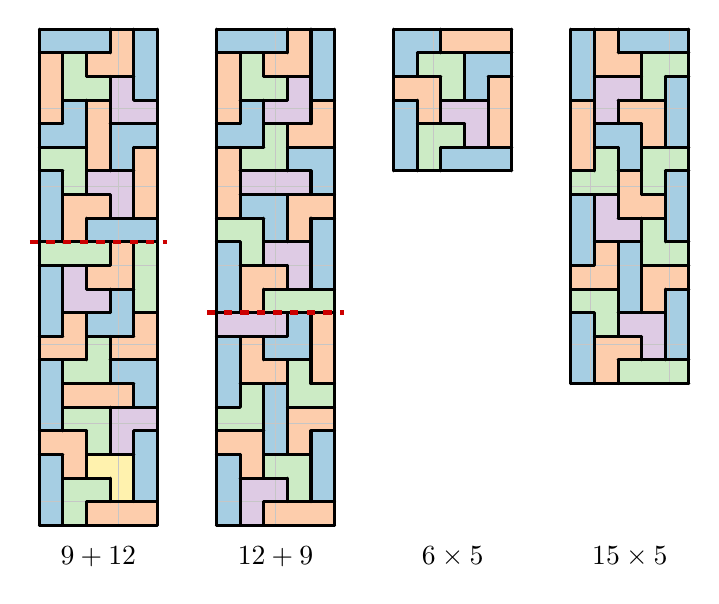
\begin{tikzpicture}[x=0.3cm,y=0.3cm]
\fill[tileA] (0,0) rectangle ++(1,-1);
\fill[tileA] (1,0) rectangle ++(1,-1);
\fill[tileA] (2,0) rectangle ++(1,-1);
\fill[tileB] (3,0) rectangle ++(1,-1);
\fill[tileB] (2,-1) rectangle ++(1,-1);
\fill[tileB] (3,-1) rectangle ++(1,-1);
\fill[tileA] (4,0) rectangle ++(1,-1);
\fill[tileA] (4,-1) rectangle ++(1,-1);
\fill[tileA] (4,-2) rectangle ++(1,-1);
\fill[tileB] (0,-1) rectangle ++(1,-1);
\fill[tileB] (0,-2) rectangle ++(1,-1);
\fill[tileB] (0,-3) rectangle ++(1,-1);
\fill[tileC] (1,-1) rectangle ++(1,-1);
\fill[tileC] (1,-2) rectangle ++(1,-1);
\fill[tileC] (2,-2) rectangle ++(1,-1);
\fill[tileD] (3,-2) rectangle ++(1,-1);
\fill[tileD] (3,-3) rectangle ++(1,-1);
\fill[tileD] (4,-3) rectangle ++(1,-1);
\fill[tileA] (1,-3) rectangle ++(1,-1);
\fill[tileA] (0,-4) rectangle ++(1,-1);
\fill[tileA] (1,-4) rectangle ++(1,-1);
\fill[tileB] (2,-3) rectangle ++(1,-1);
\fill[tileB] (2,-4) rectangle ++(1,-1);
\fill[tileB] (2,-5) rectangle ++(1,-1);
\fill[tileA] (3,-4) rectangle ++(1,-1);
\fill[tileA] (4,-4) rectangle ++(1,-1);
\fill[tileA] (3,-5) rectangle ++(1,-1);
\fill[tileC] (0,-5) rectangle ++(1,-1);
\fill[tileC] (1,-5) rectangle ++(1,-1);
\fill[tileC] (1,-6) rectangle ++(1,-1);
\fill[tileB] (4,-5) rectangle ++(1,-1);
\fill[tileB] (4,-6) rectangle ++(1,-1);
\fill[tileB] (4,-7) rectangle ++(1,-1);
\fill[tileA] (0,-6) rectangle ++(1,-1);
\fill[tileA] (0,-7) rectangle ++(1,-1);
\fill[tileA] (0,-8) rectangle ++(1,-1);
\fill[tileD] (2,-6) rectangle ++(1,-1);
\fill[tileD] (3,-6) rectangle ++(1,-1);
\fill[tileD] (3,-7) rectangle ++(1,-1);
\fill[tileB] (1,-7) rectangle ++(1,-1);
\fill[tileB] (2,-7) rectangle ++(1,-1);
\fill[tileB] (1,-8) rectangle ++(1,-1);
\fill[tileA] (2,-8) rectangle ++(1,-1);
\fill[tileA] (3,-8) rectangle ++(1,-1);
\fill[tileA] (4,-8) rectangle ++(1,-1);
\fill[tileC] (0,-9) rectangle ++(1,-1);
\fill[tileC] (1,-9) rectangle ++(1,-1);
\fill[tileC] (2,-9) rectangle ++(1,-1);
\fill[tileB] (3,-9) rectangle ++(1,-1);
\fill[tileB] (2,-10) rectangle ++(1,-1);
\fill[tileB] (3,-10) rectangle ++(1,-1);
\fill[tileC] (4,-9) rectangle ++(1,-1);
\fill[tileC] (4,-10) rectangle ++(1,-1);
\fill[tileC] (4,-11) rectangle ++(1,-1);
\fill[tileA] (0,-10) rectangle ++(1,-1);
\fill[tileA] (0,-11) rectangle ++(1,-1);
\fill[tileA] (0,-12) rectangle ++(1,-1);
\fill[tileD] (1,-10) rectangle ++(1,-1);
\fill[tileD] (1,-11) rectangle ++(1,-1);
\fill[tileD] (2,-11) rectangle ++(1,-1);
\fill[tileA] (3,-11) rectangle ++(1,-1);
\fill[tileA] (2,-12) rectangle ++(1,-1);
\fill[tileA] (3,-12) rectangle ++(1,-1);
\fill[tileB] (1,-12) rectangle ++(1,-1);
\fill[tileB] (0,-13) rectangle ++(1,-1);
\fill[tileB] (1,-13) rectangle ++(1,-1);
\fill[tileB] (4,-12) rectangle ++(1,-1);
\fill[tileB] (3,-13) rectangle ++(1,-1);
\fill[tileB] (4,-13) rectangle ++(1,-1);
\fill[tileC] (2,-13) rectangle ++(1,-1);
\fill[tileC] (1,-14) rectangle ++(1,-1);
\fill[tileC] (2,-14) rectangle ++(1,-1);
\fill[tileA] (0,-14) rectangle ++(1,-1);
\fill[tileA] (0,-15) rectangle ++(1,-1);
\fill[tileA] (0,-16) rectangle ++(1,-1);
\fill[tileA] (3,-14) rectangle ++(1,-1);
\fill[tileA] (4,-14) rectangle ++(1,-1);
\fill[tileA] (4,-15) rectangle ++(1,-1);
\fill[tileB] (1,-15) rectangle ++(1,-1);
\fill[tileB] (2,-15) rectangle ++(1,-1);
\fill[tileB] (3,-15) rectangle ++(1,-1);
\fill[tileC] (1,-16) rectangle ++(1,-1);
\fill[tileC] (2,-16) rectangle ++(1,-1);
\fill[tileC] (2,-17) rectangle ++(1,-1);
\fill[tileD] (3,-16) rectangle ++(1,-1);
\fill[tileD] (4,-16) rectangle ++(1,-1);
\fill[tileD] (3,-17) rectangle ++(1,-1);
\fill[tileB] (0,-17) rectangle ++(1,-1);
\fill[tileB] (1,-17) rectangle ++(1,-1);
\fill[tileB] (1,-18) rectangle ++(1,-1);
\fill[tileA] (4,-17) rectangle ++(1,-1);
\fill[tileA] (4,-18) rectangle ++(1,-1);
\fill[tileA] (4,-19) rectangle ++(1,-1);
\fill[tileA] (0,-18) rectangle ++(1,-1);
\fill[tileA] (0,-19) rectangle ++(1,-1);
\fill[tileA] (0,-20) rectangle ++(1,-1);
\fill[tileE] (2,-18) rectangle ++(1,-1);
\fill[tileE] (3,-18) rectangle ++(1,-1);
\fill[tileE] (3,-19) rectangle ++(1,-1);
\fill[tileC] (1,-19) rectangle ++(1,-1);
\fill[tileC] (2,-19) rectangle ++(1,-1);
\fill[tileC] (1,-20) rectangle ++(1,-1);
\fill[tileB] (2,-20) rectangle ++(1,-1);
\fill[tileB] (3,-20) rectangle ++(1,-1);
\fill[tileB] (4,-20) rectangle ++(1,-1);
\draw[cellgrid] (0,0) grid (5,-21);
\draw[tileedge] (0,-1)--++(1,0) (1,-1)--++(1,0) (3,0)--++(0,-1) (2,-1)--++(1,0) (4,0)--++(0,-1) (5,0)--++(0,-1) (1,-1)--++(0,-1) (2,-1)--++(0,-1);
\draw[tileedge] (2,-2)--++(1,0) (4,-1)--++(0,-1) (3,-2)--++(1,0) (5,-1)--++(0,-1) (1,-2)--++(0,-1) (1,-3)--++(1,0) (3,-2)--++(0,-1) (2,-3)--++(1,0);
\draw[tileedge] (4,-2)--++(0,-1) (5,-2)--++(0,-1) (4,-3)--++(1,0) (1,-3)--++(0,-1) (0,-4)--++(1,0) (2,-3)--++(0,-1) (3,-3)--++(0,-1) (3,-4)--++(1,0);
\draw[tileedge] (5,-3)--++(0,-1) (4,-4)--++(1,0) (0,-5)--++(1,0) (2,-4)--++(0,-1) (1,-5)--++(1,0) (3,-4)--++(0,-1) (5,-4)--++(0,-1) (4,-5)--++(1,0);
\draw[tileedge] (0,-6)--++(1,0) (2,-5)--++(0,-1) (3,-5)--++(0,-1) (2,-6)--++(1,0) (4,-5)--++(0,-1) (3,-6)--++(1,0) (5,-5)--++(0,-1) (1,-6)--++(0,-1);
\draw[tileedge] (2,-6)--++(0,-1) (1,-7)--++(1,0) (2,-7)--++(1,0) (4,-6)--++(0,-1) (5,-6)--++(0,-1) (1,-7)--++(0,-1) (3,-7)--++(0,-1) (2,-8)--++(1,0);
\draw[tileedge] (4,-7)--++(0,-1) (3,-8)--++(1,0) (5,-7)--++(0,-1) (4,-8)--++(1,0) (1,-8)--++(0,-1) (0,-9)--++(1,0) (2,-8)--++(0,-1) (1,-9)--++(1,0);
\draw[tileedge] (2,-9)--++(1,0) (3,-9)--++(1,0) (5,-8)--++(0,-1) (4,-9)--++(1,0) (0,-10)--++(1,0) (1,-10)--++(1,0) (3,-9)--++(0,-1) (2,-10)--++(1,0);
\draw[tileedge] (4,-9)--++(0,-1) (5,-9)--++(0,-1) (1,-10)--++(0,-1) (2,-10)--++(0,-1) (2,-11)--++(1,0) (4,-10)--++(0,-1) (3,-11)--++(1,0) (5,-10)--++(0,-1);
\draw[tileedge] (1,-11)--++(0,-1) (1,-12)--++(1,0) (3,-11)--++(0,-1) (2,-12)--++(1,0) (4,-11)--++(0,-1) (5,-11)--++(0,-1) (4,-12)--++(1,0) (1,-12)--++(0,-1);
\draw[tileedge] (0,-13)--++(1,0) (2,-12)--++(0,-1) (2,-13)--++(1,0) (4,-12)--++(0,-1) (3,-13)--++(1,0) (5,-12)--++(0,-1) (0,-14)--++(1,0) (2,-13)--++(0,-1);
\draw[tileedge] (1,-14)--++(1,0) (3,-13)--++(0,-1) (3,-14)--++(1,0) (5,-13)--++(0,-1) (4,-14)--++(1,0) (1,-14)--++(0,-1) (1,-15)--++(1,0) (3,-14)--++(0,-1);
\draw[tileedge] (2,-15)--++(1,0) (3,-15)--++(1,0) (5,-14)--++(0,-1) (1,-15)--++(0,-1) (1,-16)--++(1,0) (2,-16)--++(1,0) (4,-15)--++(0,-1) (3,-16)--++(1,0);
\draw[tileedge] (5,-15)--++(0,-1) (4,-16)--++(1,0) (1,-16)--++(0,-1) (0,-17)--++(1,0) (1,-17)--++(1,0) (3,-16)--++(0,-1) (5,-16)--++(0,-1) (4,-17)--++(1,0);
\draw[tileedge] (0,-18)--++(1,0) (2,-17)--++(0,-1) (3,-17)--++(0,-1) (2,-18)--++(1,0) (4,-17)--++(0,-1) (3,-18)--++(1,0) (5,-17)--++(0,-1) (1,-18)--++(0,-1);
\draw[tileedge] (2,-18)--++(0,-1) (1,-19)--++(1,0) (2,-19)--++(1,0) (4,-18)--++(0,-1) (5,-18)--++(0,-1) (1,-19)--++(0,-1) (3,-19)--++(0,-1) (2,-20)--++(1,0);
\draw[tileedge] (4,-19)--++(0,-1) (3,-20)--++(1,0) (5,-19)--++(0,-1) (4,-20)--++(1,0) (1,-20)--++(0,-1) (0,-21)--++(1,0) (2,-20)--++(0,-1) (1,-21)--++(1,0);
\draw[tileedge] (2,-21)--++(1,0) (3,-21)--++(1,0) (5,-20)--++(0,-1) (4,-21)--++(1,0) (0,0)--++(0,-1) (0,-1)--++(0,-1) (0,-2)--++(0,-1) (0,-3)--++(0,-1);
\draw[tileedge] (0,-4)--++(0,-1) (0,-5)--++(0,-1) (0,-6)--++(0,-1) (0,-7)--++(0,-1) (0,-8)--++(0,-1) (0,-9)--++(0,-1) (0,-10)--++(0,-1) (0,-11)--++(0,-1);
\draw[tileedge] (0,-12)--++(0,-1) (0,-13)--++(0,-1) (0,-14)--++(0,-1) (0,-15)--++(0,-1) (0,-16)--++(0,-1) (0,-17)--++(0,-1) (0,-18)--++(0,-1) (0,-19)--++(0,-1);
\draw[tileedge] (0,-20)--++(0,-1) (0,0)--++(1,0) (1,0)--++(1,0) (2,0)--++(1,0) (3,0)--++(1,0) (4,0)--++(1,0);
\draw[seam] (-0.4,-9)--(5.4,-9);
\node[below] at (2.5,-21.5) {$9+12$};
\fill[tileA] (7.5,0) rectangle ++(1,-1);
\fill[tileA] (8.5,0) rectangle ++(1,-1);
\fill[tileA] (9.5,0) rectangle ++(1,-1);
\fill[tileB] (10.5,0) rectangle ++(1,-1);
\fill[tileB] (9.5,-1) rectangle ++(1,-1);
\fill[tileB] (10.5,-1) rectangle ++(1,-1);
\fill[tileA] (11.5,0) rectangle ++(1,-1);
\fill[tileA] (11.5,-1) rectangle ++(1,-1);
\fill[tileA] (11.5,-2) rectangle ++(1,-1);
\fill[tileB] (7.5,-1) rectangle ++(1,-1);
\fill[tileB] (7.5,-2) rectangle ++(1,-1);
\fill[tileB] (7.5,-3) rectangle ++(1,-1);
\fill[tileC] (8.5,-1) rectangle ++(1,-1);
\fill[tileC] (8.5,-2) rectangle ++(1,-1);
\fill[tileC] (9.5,-2) rectangle ++(1,-1);
\fill[tileD] (10.5,-2) rectangle ++(1,-1);
\fill[tileD] (9.5,-3) rectangle ++(1,-1);
\fill[tileD] (10.5,-3) rectangle ++(1,-1);
\fill[tileA] (8.5,-3) rectangle ++(1,-1);
\fill[tileA] (7.5,-4) rectangle ++(1,-1);
\fill[tileA] (8.5,-4) rectangle ++(1,-1);
\fill[tileB] (11.5,-3) rectangle ++(1,-1);
\fill[tileB] (10.5,-4) rectangle ++(1,-1);
\fill[tileB] (11.5,-4) rectangle ++(1,-1);
\fill[tileC] (9.5,-4) rectangle ++(1,-1);
\fill[tileC] (8.5,-5) rectangle ++(1,-1);
\fill[tileC] (9.5,-5) rectangle ++(1,-1);
\fill[tileB] (7.5,-5) rectangle ++(1,-1);
\fill[tileB] (7.5,-6) rectangle ++(1,-1);
\fill[tileB] (7.5,-7) rectangle ++(1,-1);
\fill[tileA] (10.5,-5) rectangle ++(1,-1);
\fill[tileA] (11.5,-5) rectangle ++(1,-1);
\fill[tileA] (11.5,-6) rectangle ++(1,-1);
\fill[tileD] (8.5,-6) rectangle ++(1,-1);
\fill[tileD] (9.5,-6) rectangle ++(1,-1);
\fill[tileD] (10.5,-6) rectangle ++(1,-1);
\fill[tileA] (8.5,-7) rectangle ++(1,-1);
\fill[tileA] (9.5,-7) rectangle ++(1,-1);
\fill[tileA] (9.5,-8) rectangle ++(1,-1);
\fill[tileB] (10.5,-7) rectangle ++(1,-1);
\fill[tileB] (11.5,-7) rectangle ++(1,-1);
\fill[tileB] (10.5,-8) rectangle ++(1,-1);
\fill[tileC] (7.5,-8) rectangle ++(1,-1);
\fill[tileC] (8.5,-8) rectangle ++(1,-1);
\fill[tileC] (8.5,-9) rectangle ++(1,-1);
\fill[tileA] (11.5,-8) rectangle ++(1,-1);
\fill[tileA] (11.5,-9) rectangle ++(1,-1);
\fill[tileA] (11.5,-10) rectangle ++(1,-1);
\fill[tileA] (7.5,-9) rectangle ++(1,-1);
\fill[tileA] (7.5,-10) rectangle ++(1,-1);
\fill[tileA] (7.5,-11) rectangle ++(1,-1);
\fill[tileD] (9.5,-9) rectangle ++(1,-1);
\fill[tileD] (10.5,-9) rectangle ++(1,-1);
\fill[tileD] (10.5,-10) rectangle ++(1,-1);
\fill[tileB] (8.5,-10) rectangle ++(1,-1);
\fill[tileB] (9.5,-10) rectangle ++(1,-1);
\fill[tileB] (8.5,-11) rectangle ++(1,-1);
\fill[tileC] (9.5,-11) rectangle ++(1,-1);
\fill[tileC] (10.5,-11) rectangle ++(1,-1);
\fill[tileC] (11.5,-11) rectangle ++(1,-1);
\fill[tileD] (7.5,-12) rectangle ++(1,-1);
\fill[tileD] (8.5,-12) rectangle ++(1,-1);
\fill[tileD] (9.5,-12) rectangle ++(1,-1);
\fill[tileA] (10.5,-12) rectangle ++(1,-1);
\fill[tileA] (9.5,-13) rectangle ++(1,-1);
\fill[tileA] (10.5,-13) rectangle ++(1,-1);
\fill[tileB] (11.5,-12) rectangle ++(1,-1);
\fill[tileB] (11.5,-13) rectangle ++(1,-1);
\fill[tileB] (11.5,-14) rectangle ++(1,-1);
\fill[tileA] (7.5,-13) rectangle ++(1,-1);
\fill[tileA] (7.5,-14) rectangle ++(1,-1);
\fill[tileA] (7.5,-15) rectangle ++(1,-1);
\fill[tileB] (8.5,-13) rectangle ++(1,-1);
\fill[tileB] (8.5,-14) rectangle ++(1,-1);
\fill[tileB] (9.5,-14) rectangle ++(1,-1);
\fill[tileC] (10.5,-14) rectangle ++(1,-1);
\fill[tileC] (10.5,-15) rectangle ++(1,-1);
\fill[tileC] (11.5,-15) rectangle ++(1,-1);
\fill[tileC] (8.5,-15) rectangle ++(1,-1);
\fill[tileC] (7.5,-16) rectangle ++(1,-1);
\fill[tileC] (8.5,-16) rectangle ++(1,-1);
\fill[tileA] (9.5,-15) rectangle ++(1,-1);
\fill[tileA] (9.5,-16) rectangle ++(1,-1);
\fill[tileA] (9.5,-17) rectangle ++(1,-1);
\fill[tileB] (10.5,-16) rectangle ++(1,-1);
\fill[tileB] (11.5,-16) rectangle ++(1,-1);
\fill[tileB] (10.5,-17) rectangle ++(1,-1);
\fill[tileB] (7.5,-17) rectangle ++(1,-1);
\fill[tileB] (8.5,-17) rectangle ++(1,-1);
\fill[tileB] (8.5,-18) rectangle ++(1,-1);
\fill[tileA] (11.5,-17) rectangle ++(1,-1);
\fill[tileA] (11.5,-18) rectangle ++(1,-1);
\fill[tileA] (11.5,-19) rectangle ++(1,-1);
\fill[tileA] (7.5,-18) rectangle ++(1,-1);
\fill[tileA] (7.5,-19) rectangle ++(1,-1);
\fill[tileA] (7.5,-20) rectangle ++(1,-1);
\fill[tileC] (9.5,-18) rectangle ++(1,-1);
\fill[tileC] (10.5,-18) rectangle ++(1,-1);
\fill[tileC] (10.5,-19) rectangle ++(1,-1);
\fill[tileD] (8.5,-19) rectangle ++(1,-1);
\fill[tileD] (9.5,-19) rectangle ++(1,-1);
\fill[tileD] (8.5,-20) rectangle ++(1,-1);
\fill[tileB] (9.5,-20) rectangle ++(1,-1);
\fill[tileB] (10.5,-20) rectangle ++(1,-1);
\fill[tileB] (11.5,-20) rectangle ++(1,-1);
\draw[cellgrid] (7.5,0) grid (12.5,-21);
\draw[tileedge] (7.5,-1)--++(1,0) (8.5,-1)--++(1,0) (10.5,0)--++(0,-1) (9.5,-1)--++(1,0) (11.5,0)--++(0,-1) (12.5,0)--++(0,-1) (8.5,-1)--++(0,-1) (9.5,-1)--++(0,-1);
\draw[tileedge] (9.5,-2)--++(1,0) (11.5,-1)--++(0,-1) (10.5,-2)--++(1,0) (12.5,-1)--++(0,-1) (8.5,-2)--++(0,-1) (8.5,-3)--++(1,0) (10.5,-2)--++(0,-1) (9.5,-3)--++(1,0);
\draw[tileedge] (11.5,-2)--++(0,-1) (12.5,-2)--++(0,-1) (11.5,-3)--++(1,0) (8.5,-3)--++(0,-1) (7.5,-4)--++(1,0) (9.5,-3)--++(0,-1) (9.5,-4)--++(1,0) (11.5,-3)--++(0,-1);
\draw[tileedge] (10.5,-4)--++(1,0) (12.5,-3)--++(0,-1) (7.5,-5)--++(1,0) (9.5,-4)--++(0,-1) (8.5,-5)--++(1,0) (10.5,-4)--++(0,-1) (10.5,-5)--++(1,0) (12.5,-4)--++(0,-1);
\draw[tileedge] (11.5,-5)--++(1,0) (8.5,-5)--++(0,-1) (8.5,-6)--++(1,0) (10.5,-5)--++(0,-1) (9.5,-6)--++(1,0) (10.5,-6)--++(1,0) (12.5,-5)--++(0,-1) (8.5,-6)--++(0,-1);
\draw[tileedge] (8.5,-7)--++(1,0) (9.5,-7)--++(1,0) (11.5,-6)--++(0,-1) (10.5,-7)--++(1,0) (12.5,-6)--++(0,-1) (11.5,-7)--++(1,0) (8.5,-7)--++(0,-1) (7.5,-8)--++(1,0);
\draw[tileedge] (8.5,-8)--++(1,0) (10.5,-7)--++(0,-1) (12.5,-7)--++(0,-1) (11.5,-8)--++(1,0) (7.5,-9)--++(1,0) (9.5,-8)--++(0,-1) (10.5,-8)--++(0,-1) (9.5,-9)--++(1,0);
\draw[tileedge] (11.5,-8)--++(0,-1) (10.5,-9)--++(1,0) (12.5,-8)--++(0,-1) (8.5,-9)--++(0,-1) (9.5,-9)--++(0,-1) (8.5,-10)--++(1,0) (9.5,-10)--++(1,0) (11.5,-9)--++(0,-1);
\draw[tileedge] (12.5,-9)--++(0,-1) (8.5,-10)--++(0,-1) (10.5,-10)--++(0,-1) (9.5,-11)--++(1,0) (11.5,-10)--++(0,-1) (10.5,-11)--++(1,0) (12.5,-10)--++(0,-1) (11.5,-11)--++(1,0);
\draw[tileedge] (8.5,-11)--++(0,-1) (7.5,-12)--++(1,0) (9.5,-11)--++(0,-1) (8.5,-12)--++(1,0) (9.5,-12)--++(1,0) (10.5,-12)--++(1,0) (12.5,-11)--++(0,-1) (11.5,-12)--++(1,0);
\draw[tileedge] (7.5,-13)--++(1,0) (8.5,-13)--++(1,0) (10.5,-12)--++(0,-1) (9.5,-13)--++(1,0) (11.5,-12)--++(0,-1) (12.5,-12)--++(0,-1) (8.5,-13)--++(0,-1) (9.5,-13)--++(0,-1);
\draw[tileedge] (9.5,-14)--++(1,0) (11.5,-13)--++(0,-1) (10.5,-14)--++(1,0) (12.5,-13)--++(0,-1) (8.5,-14)--++(0,-1) (8.5,-15)--++(1,0) (10.5,-14)--++(0,-1) (9.5,-15)--++(1,0);
\draw[tileedge] (11.5,-14)--++(0,-1) (12.5,-14)--++(0,-1) (11.5,-15)--++(1,0) (8.5,-15)--++(0,-1) (7.5,-16)--++(1,0) (9.5,-15)--++(0,-1) (10.5,-15)--++(0,-1) (10.5,-16)--++(1,0);
\draw[tileedge] (12.5,-15)--++(0,-1) (11.5,-16)--++(1,0) (7.5,-17)--++(1,0) (9.5,-16)--++(0,-1) (8.5,-17)--++(1,0) (10.5,-16)--++(0,-1) (12.5,-16)--++(0,-1) (11.5,-17)--++(1,0);
\draw[tileedge] (7.5,-18)--++(1,0) (9.5,-17)--++(0,-1) (10.5,-17)--++(0,-1) (9.5,-18)--++(1,0) (11.5,-17)--++(0,-1) (10.5,-18)--++(1,0) (12.5,-17)--++(0,-1) (8.5,-18)--++(0,-1);
\draw[tileedge] (9.5,-18)--++(0,-1) (8.5,-19)--++(1,0) (9.5,-19)--++(1,0) (11.5,-18)--++(0,-1) (12.5,-18)--++(0,-1) (8.5,-19)--++(0,-1) (10.5,-19)--++(0,-1) (9.5,-20)--++(1,0);
\draw[tileedge] (11.5,-19)--++(0,-1) (10.5,-20)--++(1,0) (12.5,-19)--++(0,-1) (11.5,-20)--++(1,0) (8.5,-20)--++(0,-1) (7.5,-21)--++(1,0) (9.5,-20)--++(0,-1) (8.5,-21)--++(1,0);
\draw[tileedge] (9.5,-21)--++(1,0) (10.5,-21)--++(1,0) (12.5,-20)--++(0,-1) (11.5,-21)--++(1,0) (7.5,0)--++(0,-1) (7.5,-1)--++(0,-1) (7.5,-2)--++(0,-1) (7.5,-3)--++(0,-1);
\draw[tileedge] (7.5,-4)--++(0,-1) (7.5,-5)--++(0,-1) (7.5,-6)--++(0,-1) (7.5,-7)--++(0,-1) (7.5,-8)--++(0,-1) (7.5,-9)--++(0,-1) (7.5,-10)--++(0,-1) (7.5,-11)--++(0,-1);
\draw[tileedge] (7.5,-12)--++(0,-1) (7.5,-13)--++(0,-1) (7.5,-14)--++(0,-1) (7.5,-15)--++(0,-1) (7.5,-16)--++(0,-1) (7.5,-17)--++(0,-1) (7.5,-18)--++(0,-1) (7.5,-19)--++(0,-1);
\draw[tileedge] (7.5,-20)--++(0,-1) (7.5,0)--++(1,0) (8.5,0)--++(1,0) (9.5,0)--++(1,0) (10.5,0)--++(1,0) (11.5,0)--++(1,0);
\draw[seam] (7.1,-12)--(12.9,-12);
\node[below] at (10,-21.5) {$12+9$};
\fill[tileA] (15,0) rectangle ++(1,-1);
\fill[tileA] (16,0) rectangle ++(1,-1);
\fill[tileA] (15,-1) rectangle ++(1,-1);
\fill[tileB] (17,0) rectangle ++(1,-1);
\fill[tileB] (18,0) rectangle ++(1,-1);
\fill[tileB] (19,0) rectangle ++(1,-1);
\fill[tileC] (16,-1) rectangle ++(1,-1);
\fill[tileC] (17,-1) rectangle ++(1,-1);
\fill[tileC] (17,-2) rectangle ++(1,-1);
\fill[tileA] (18,-1) rectangle ++(1,-1);
\fill[tileA] (19,-1) rectangle ++(1,-1);
\fill[tileA] (18,-2) rectangle ++(1,-1);
\fill[tileB] (15,-2) rectangle ++(1,-1);
\fill[tileB] (16,-2) rectangle ++(1,-1);
\fill[tileB] (16,-3) rectangle ++(1,-1);
\fill[tileB] (19,-2) rectangle ++(1,-1);
\fill[tileB] (19,-3) rectangle ++(1,-1);
\fill[tileB] (19,-4) rectangle ++(1,-1);
\fill[tileA] (15,-3) rectangle ++(1,-1);
\fill[tileA] (15,-4) rectangle ++(1,-1);
\fill[tileA] (15,-5) rectangle ++(1,-1);
\fill[tileD] (17,-3) rectangle ++(1,-1);
\fill[tileD] (18,-3) rectangle ++(1,-1);
\fill[tileD] (18,-4) rectangle ++(1,-1);
\fill[tileC] (16,-4) rectangle ++(1,-1);
\fill[tileC] (17,-4) rectangle ++(1,-1);
\fill[tileC] (16,-5) rectangle ++(1,-1);
\fill[tileA] (17,-5) rectangle ++(1,-1);
\fill[tileA] (18,-5) rectangle ++(1,-1);
\fill[tileA] (19,-5) rectangle ++(1,-1);
\draw[cellgrid] (15,0) grid (20,-6);
\draw[tileedge] (17,0)--++(0,-1) (16,-1)--++(1,0) (17,-1)--++(1,0) (18,-1)--++(1,0) (20,0)--++(0,-1) (19,-1)--++(1,0) (16,-1)--++(0,-1) (15,-2)--++(1,0);
\draw[tileedge] (16,-2)--++(1,0) (18,-1)--++(0,-1) (20,-1)--++(0,-1) (19,-2)--++(1,0) (15,-3)--++(1,0) (17,-2)--++(0,-1) (18,-2)--++(0,-1) (17,-3)--++(1,0);
\draw[tileedge] (19,-2)--++(0,-1) (18,-3)--++(1,0) (20,-2)--++(0,-1) (16,-3)--++(0,-1) (17,-3)--++(0,-1) (16,-4)--++(1,0) (17,-4)--++(1,0) (19,-3)--++(0,-1);
\draw[tileedge] (20,-3)--++(0,-1) (16,-4)--++(0,-1) (18,-4)--++(0,-1) (17,-5)--++(1,0) (19,-4)--++(0,-1) (18,-5)--++(1,0) (20,-4)--++(0,-1) (19,-5)--++(1,0);
\draw[tileedge] (16,-5)--++(0,-1) (15,-6)--++(1,0) (17,-5)--++(0,-1) (16,-6)--++(1,0) (17,-6)--++(1,0) (18,-6)--++(1,0) (20,-5)--++(0,-1) (19,-6)--++(1,0);
\draw[tileedge] (15,0)--++(0,-1) (15,-1)--++(0,-1) (15,-2)--++(0,-1) (15,-3)--++(0,-1) (15,-4)--++(0,-1) (15,-5)--++(0,-1) (15,0)--++(1,0) (16,0)--++(1,0);
\draw[tileedge] (17,0)--++(1,0) (18,0)--++(1,0) (19,0)--++(1,0);
\node[below] at (17.5,-21.5) {$6\times5$};
\fill[tileA] (22.5,0) rectangle ++(1,-1);
\fill[tileA] (22.5,-1) rectangle ++(1,-1);
\fill[tileA] (22.5,-2) rectangle ++(1,-1);
\fill[tileB] (23.5,0) rectangle ++(1,-1);
\fill[tileB] (23.5,-1) rectangle ++(1,-1);
\fill[tileB] (24.5,-1) rectangle ++(1,-1);
\fill[tileA] (24.5,0) rectangle ++(1,-1);
\fill[tileA] (25.5,0) rectangle ++(1,-1);
\fill[tileA] (26.5,0) rectangle ++(1,-1);
\fill[tileC] (25.5,-1) rectangle ++(1,-1);
\fill[tileC] (26.5,-1) rectangle ++(1,-1);
\fill[tileC] (25.5,-2) rectangle ++(1,-1);
\fill[tileD] (23.5,-2) rectangle ++(1,-1);
\fill[tileD] (24.5,-2) rectangle ++(1,-1);
\fill[tileD] (23.5,-3) rectangle ++(1,-1);
\fill[tileA] (26.5,-2) rectangle ++(1,-1);
\fill[tileA] (26.5,-3) rectangle ++(1,-1);
\fill[tileA] (26.5,-4) rectangle ++(1,-1);
\fill[tileB] (22.5,-3) rectangle ++(1,-1);
\fill[tileB] (22.5,-4) rectangle ++(1,-1);
\fill[tileB] (22.5,-5) rectangle ++(1,-1);
\fill[tileB] (24.5,-3) rectangle ++(1,-1);
\fill[tileB] (25.5,-3) rectangle ++(1,-1);
\fill[tileB] (25.5,-4) rectangle ++(1,-1);
\fill[tileA] (23.5,-4) rectangle ++(1,-1);
\fill[tileA] (24.5,-4) rectangle ++(1,-1);
\fill[tileA] (24.5,-5) rectangle ++(1,-1);
\fill[tileC] (23.5,-5) rectangle ++(1,-1);
\fill[tileC] (22.5,-6) rectangle ++(1,-1);
\fill[tileC] (23.5,-6) rectangle ++(1,-1);
\fill[tileC] (25.5,-5) rectangle ++(1,-1);
\fill[tileC] (26.5,-5) rectangle ++(1,-1);
\fill[tileC] (25.5,-6) rectangle ++(1,-1);
\fill[tileB] (24.5,-6) rectangle ++(1,-1);
\fill[tileB] (24.5,-7) rectangle ++(1,-1);
\fill[tileB] (25.5,-7) rectangle ++(1,-1);
\fill[tileA] (26.5,-6) rectangle ++(1,-1);
\fill[tileA] (26.5,-7) rectangle ++(1,-1);
\fill[tileA] (26.5,-8) rectangle ++(1,-1);
\fill[tileA] (22.5,-7) rectangle ++(1,-1);
\fill[tileA] (22.5,-8) rectangle ++(1,-1);
\fill[tileA] (22.5,-9) rectangle ++(1,-1);
\fill[tileD] (23.5,-7) rectangle ++(1,-1);
\fill[tileD] (23.5,-8) rectangle ++(1,-1);
\fill[tileD] (24.5,-8) rectangle ++(1,-1);
\fill[tileC] (25.5,-8) rectangle ++(1,-1);
\fill[tileC] (25.5,-9) rectangle ++(1,-1);
\fill[tileC] (26.5,-9) rectangle ++(1,-1);
\fill[tileB] (23.5,-9) rectangle ++(1,-1);
\fill[tileB] (22.5,-10) rectangle ++(1,-1);
\fill[tileB] (23.5,-10) rectangle ++(1,-1);
\fill[tileA] (24.5,-9) rectangle ++(1,-1);
\fill[tileA] (24.5,-10) rectangle ++(1,-1);
\fill[tileA] (24.5,-11) rectangle ++(1,-1);
\fill[tileB] (25.5,-10) rectangle ++(1,-1);
\fill[tileB] (26.5,-10) rectangle ++(1,-1);
\fill[tileB] (25.5,-11) rectangle ++(1,-1);
\fill[tileC] (22.5,-11) rectangle ++(1,-1);
\fill[tileC] (23.5,-11) rectangle ++(1,-1);
\fill[tileC] (23.5,-12) rectangle ++(1,-1);
\fill[tileA] (26.5,-11) rectangle ++(1,-1);
\fill[tileA] (26.5,-12) rectangle ++(1,-1);
\fill[tileA] (26.5,-13) rectangle ++(1,-1);
\fill[tileA] (22.5,-12) rectangle ++(1,-1);
\fill[tileA] (22.5,-13) rectangle ++(1,-1);
\fill[tileA] (22.5,-14) rectangle ++(1,-1);
\fill[tileD] (24.5,-12) rectangle ++(1,-1);
\fill[tileD] (25.5,-12) rectangle ++(1,-1);
\fill[tileD] (25.5,-13) rectangle ++(1,-1);
\fill[tileB] (23.5,-13) rectangle ++(1,-1);
\fill[tileB] (24.5,-13) rectangle ++(1,-1);
\fill[tileB] (23.5,-14) rectangle ++(1,-1);
\fill[tileC] (24.5,-14) rectangle ++(1,-1);
\fill[tileC] (25.5,-14) rectangle ++(1,-1);
\fill[tileC] (26.5,-14) rectangle ++(1,-1);
\draw[cellgrid] (22.5,0) grid (27.5,-15);
\draw[tileedge] (23.5,0)--++(0,-1) (24.5,0)--++(0,-1) (24.5,-1)--++(1,0) (25.5,-1)--++(1,0) (27.5,0)--++(0,-1) (26.5,-1)--++(1,0) (23.5,-1)--++(0,-1) (23.5,-2)--++(1,0);
\draw[tileedge] (25.5,-1)--++(0,-1) (24.5,-2)--++(1,0) (27.5,-1)--++(0,-1) (26.5,-2)--++(1,0) (23.5,-2)--++(0,-1) (22.5,-3)--++(1,0) (25.5,-2)--++(0,-1) (24.5,-3)--++(1,0);
\draw[tileedge] (26.5,-2)--++(0,-1) (25.5,-3)--++(1,0) (27.5,-2)--++(0,-1) (23.5,-3)--++(0,-1) (24.5,-3)--++(0,-1) (23.5,-4)--++(1,0) (24.5,-4)--++(1,0) (26.5,-3)--++(0,-1);
\draw[tileedge] (27.5,-3)--++(0,-1) (23.5,-4)--++(0,-1) (23.5,-5)--++(1,0) (25.5,-4)--++(0,-1) (26.5,-4)--++(0,-1) (25.5,-5)--++(1,0) (27.5,-4)--++(0,-1) (26.5,-5)--++(1,0);
\draw[tileedge] (23.5,-5)--++(0,-1) (22.5,-6)--++(1,0) (24.5,-5)--++(0,-1) (25.5,-5)--++(0,-1) (24.5,-6)--++(1,0) (27.5,-5)--++(0,-1) (26.5,-6)--++(1,0) (22.5,-7)--++(1,0);
\draw[tileedge] (24.5,-6)--++(0,-1) (23.5,-7)--++(1,0) (25.5,-6)--++(0,-1) (26.5,-6)--++(0,-1) (25.5,-7)--++(1,0) (27.5,-6)--++(0,-1) (23.5,-7)--++(0,-1) (24.5,-7)--++(0,-1);
\draw[tileedge] (24.5,-8)--++(1,0) (26.5,-7)--++(0,-1) (25.5,-8)--++(1,0) (27.5,-7)--++(0,-1) (23.5,-8)--++(0,-1) (23.5,-9)--++(1,0) (25.5,-8)--++(0,-1) (24.5,-9)--++(1,0);
\draw[tileedge] (26.5,-8)--++(0,-1) (27.5,-8)--++(0,-1) (26.5,-9)--++(1,0) (23.5,-9)--++(0,-1) (22.5,-10)--++(1,0) (24.5,-9)--++(0,-1) (25.5,-9)--++(0,-1) (25.5,-10)--++(1,0);
\draw[tileedge] (27.5,-9)--++(0,-1) (26.5,-10)--++(1,0) (22.5,-11)--++(1,0) (24.5,-10)--++(0,-1) (23.5,-11)--++(1,0) (25.5,-10)--++(0,-1) (27.5,-10)--++(0,-1) (26.5,-11)--++(1,0);
\draw[tileedge] (22.5,-12)--++(1,0) (24.5,-11)--++(0,-1) (25.5,-11)--++(0,-1) (24.5,-12)--++(1,0) (26.5,-11)--++(0,-1) (25.5,-12)--++(1,0) (27.5,-11)--++(0,-1) (23.5,-12)--++(0,-1);
\draw[tileedge] (24.5,-12)--++(0,-1) (23.5,-13)--++(1,0) (24.5,-13)--++(1,0) (26.5,-12)--++(0,-1) (27.5,-12)--++(0,-1) (23.5,-13)--++(0,-1) (25.5,-13)--++(0,-1) (24.5,-14)--++(1,0);
\draw[tileedge] (26.5,-13)--++(0,-1) (25.5,-14)--++(1,0) (27.5,-13)--++(0,-1) (26.5,-14)--++(1,0) (23.5,-14)--++(0,-1) (22.5,-15)--++(1,0) (24.5,-14)--++(0,-1) (23.5,-15)--++(1,0);
\draw[tileedge] (24.5,-15)--++(1,0) (25.5,-15)--++(1,0) (27.5,-14)--++(0,-1) (26.5,-15)--++(1,0) (22.5,0)--++(0,-1) (22.5,-1)--++(0,-1) (22.5,-2)--++(0,-1) (22.5,-3)--++(0,-1);
\draw[tileedge] (22.5,-4)--++(0,-1) (22.5,-5)--++(0,-1) (22.5,-6)--++(0,-1) (22.5,-7)--++(0,-1) (22.5,-8)--++(0,-1) (22.5,-9)--++(0,-1) (22.5,-10)--++(0,-1) (22.5,-11)--++(0,-1);
\draw[tileedge] (22.5,-12)--++(0,-1) (22.5,-13)--++(0,-1) (22.5,-14)--++(0,-1) (22.5,0)--++(1,0) (23.5,0)--++(1,0) (24.5,0)--++(1,0) (25.5,0)--++(1,0) (26.5,0)--++(1,0);
\node[below] at (25,-21.5) {$15\times5$};
\end{tikzpicture}
%% END FIGURE width-five
\caption{Width 5. Left: the blocks $B_{9,5}$ and $B_{12,5}$ stacked in both
orders, seams dashed (each also stacks on itself). Right: the single tilings
of the $6\times5$ and $15\times5$ rectangles, the two admissible heights that are not
sums of nines and twelves.}
\label{fig:five}
\end{figure}

\end{appendices}
\clearpage

\begin{thebibliography}{9}
\bibitem{faultfree}
M.~Aanjaneya and S.~P. Pal,
\emph{Faultfree tromino tilings of rectangles},
arXiv:math/0610925, 2006.
\url{https://arxiv.org/abs/math/0610925}.

\bibitem{akitaya}
H.~A. Akitaya, K.~Dituro, A.~Gonczi, M.~Korman, D.~L. Souvaine, F.~Stock and
C.~D. T\'oth,
\emph{Redistricting in triangular and square grids},
in: 2026 Symposium on Simplicity in Algorithms (SOSA), SIAM, 2026, 12--25.
\href{https://doi.org/10.1137/1.9781611978964.2}{doi:10.1137/1.9781611978964.2}.

\bibitem{cannon}
S.~Cannon,
\emph{Irreducibility of recombination Markov chains in the triangular lattice},
Discrete Applied Mathematics \textbf{347} (2024), 75--130.
\href{https://doi.org/10.1016/j.dam.2023.12.019}{doi:10.1016/j.dam.2023.12.019}.
Theorem numbering from arXiv:2305.17239v2, December 19, 2023.
\url{https://arxiv.org/abs/2305.17239v2}.

\bibitem{recom}
D.~DeFord, M.~Duchin and J.~Solomon,
\emph{Recombination: a family of Markov chains for redistricting},
Harvard Data Science Review \textbf{3} (2021), no.~1.
\href{https://doi.org/10.1162/99608f92.eb30390f}{doi:10.1162/99608f92.eb30390f}.

\bibitem{emre}
M.~Emre, D.~C. Jerison and E.~Veomett,
\emph{Connectivity of districting metagraphs},
arXiv:2606.10152v2, September 8, 2026.
\url{https://arxiv.org/abs/2606.10152v2}.

\bibitem{GrahamArchive}
P.~Graham,
\emph{Locked tromino tilings of rectangles}, version~3,
Zenodo, 2026.
\href{https://doi.org/10.5281/zenodo.23638798}{doi:10.5281/zenodo.23638798}.

\bibitem{lean}
L.~de Moura and S.~Ullrich,
\emph{The Lean~4 theorem prover and programming language},
in: Automated Deduction -- CADE 28, Lecture Notes in Computer Science
\textbf{12699}, Springer, 2021, 625--635.
\href{https://doi.org/10.1007/978-3-030-79876-5_37}{doi:10.1007/978-3-030-79876-5\_37}.

\bibitem{tf}
J.~Tucker-Foltz,
\emph{Locked polyomino tilings},
arXiv:2307.15996v4, December 10, 2024.
\url{https://arxiv.org/abs/2307.15996v4}.
\end{thebibliography}

\end{document}
